%%%%%%%%%%%%%%%%%%%%%%%%%%%%%%%%%%%%%%%%%%%%%%%%%%%
%% LaTeX book template                           %%
%% Author:  Amber Jain (http://amberj.devio.us/) %%
%% License: ISC license                          %%
%%%%%%%%%%%%%%%%%%%%%%%%%%%%%%%%%%%%%%%%%%%%%%%%%%%

\documentclass[a4paper,11pt,oneside]{book}

% pacotes utilizados
\usepackage[T1]{fontenc}
\usepackage[utf8]{inputenc}
\usepackage{lmodern}
\usepackage{hyperref}
\usepackage{graphicx}
\usepackage[portuguese]{babel}
\usepackage{amsfonts}
\usepackage[usenames,dvipsnames]{xcolor}
\usepackage{mathtools}
\usepackage{amssymb} % alguns simbolos matematicos
\usepackage{mathrsfs} % letras cursivas
\usepackage{listings} % coding examples in latex file
\usepackage{xcolor} % changing colors
\usepackage{amsthm} % definir estilo do teorema
\usepackage[hang,flushmargin]{footmisc} % remove footnote's identation
\usepackage{cancel} % para poder colocar o tracinho de cancelamento
\usepackage{tikz} % to draw Venn's diagrams

% dark theme no pdf
\pagecolor[rgb]{0.1,0.1,0.1} %black
\color[rgb]{0.9,0.9,0.9} %grey

% criando o modelo de definicoes/teoremas/fatos/demonstracoes
\theoremstyle{definition}

\newtheoremstyle{break}% name
  {10pt}%         Space above, empty = `usual value'
  {10pt}%         Space below
  {}% Body font
  {}%         Indent amount (empty = no indent, \parindent = para indent)
  {\bfseries}% Thm head font
  {}%        Punctuation after thm head
  {\newline}% Space after thm head: \newline = linebreak
  {}%         Thm head spec

\theoremstyle{break}

% definindo as categorias de formalidade
\newtheorem{definition}{Definição}[section]
\newtheorem{fact}{Fato}[section]
\newtheorem{demonstration}{Demonstração}[section]
\newtheorem{theorem}{Teorema}
\newtheorem{proposition}{Proposição}

% tirando identação dos paragrafos
\setlength{\parindent}{0ex}

% setting das cores quando usar codigo python
\definecolor{codegreen}{rgb}{0,0.6,0}
\definecolor{codegray}{rgb}{0.5,0.5,0.5}
\definecolor{codepurple}{rgb}{0.58,0,0.82}
\definecolor{backcolour}{rgb}{0.95,0.95,0.92}

\lstdefinestyle{mystyle}{
    backgroundcolor=\color{backcolour},   
    commentstyle=\color{codegreen},
    keywordstyle=\color{magenta},
    numberstyle=\tiny\color{codegray},
    stringstyle=\color{codepurple},
    basicstyle=\ttfamily\footnotesize,
    breakatwhitespace=false,         
    breaklines=true,                 
    captionpos=b,                    
    keepspaces=true,                 
    numbers=left,                    
    numbersep=5pt,                  
    showspaces=false,                
    showstringspaces=false,
    showtabs=false,                  
    tabsize=2
}

\lstset{style=mystyle}

% dedicatoria 
% Source: http://www.tug.org/pipermail/texhax/2010-June/
\newenvironment{dedication}
{
   \cleardoublepage
   \thispagestyle{empty}
   \vspace*{\stretch{1}}
   \hfill\begin{minipage}[t]{0.66\textwidth}
   \raggedright
}
{
   \end{minipage}
   \vspace*{\stretch{3}}
   \clearpage
}

% Chapter quote at the start of chapter        %
% Source: http://tex.stackexchange.com/a/53380 %
\makeatletter
\renewcommand{\@chapapp}{}% Not necessary...
\newenvironment{chapquote}[2][2em]
  {\setlength{\@tempdima}{#1}%
   \def\chapquote@author{#2}%
   \parshape 1 \@tempdima \dimexpr\textwidth-2\@tempdima\relax%
   \itshape}
  {\par\normalfont\hfill--\ \chapquote@author\hspace*{\@tempdima}\par\bigskip}
\makeatother


%%%%%%%%%%%%%%%%%%%%%%%%%%%%%%%%%%%%%%%%%%%%%%%%%%%
% First page of book which contains 'stuff' like: %
%  - Book title, subtitle                         %
%  - Book author name                             %
%%%%%%%%%%%%%%%%%%%%%%%%%%%%%%%%%%%%%%%%%%%%%%%%%%%
% Book's title and subtitle
\title{\Huge \textbf{Book of Proof} \\ 
\Large Third Edition \\
\huge by Richard Hammack}

% Author
\author{
\textsc{Resumo e Adaptação por:} \\
\textsc{Bruno de M. Ruas} e \\ 
\textsc{Luiz Eduardo de Lima} 
}

\begin{document}

\frontmatter
\maketitle

\tableofcontents
%\listoffigures
%\listoftables

\mainmatter

%%%%%%%%%%%%%%%%%%%%%%%%%%%%%%%%%%%%%%%%%%%%%%%%%%%
%                    PART                         %
%%%%%%%%%%%%%%%%%%%%%%%%%%%%%%%%%%%%%%%%%%%%%%%%%%%
\part{Fundamentos}

%%%%%%%%%%%%%%%%%%%%%%%% CHAPTER %%%%%%%%%%%%%%%%%%%%%%%%
\chapter{Conjuntos}

\begin{chapquote}{página 3}
	``The theory of sets is a language that is perfectly suited to describing and explaning all types of mathematical structures.''
\end{chapquote}

\section*{Aviso ao Leitor}
Bem-vindo ao início de uma jornada consideravelmente longa. Esse texto é um resumo (mais conciso e menos didático) do livro do professor Hammack. O objetivo desse presente manual é servir como material de revisão e auxílio aos que quiserem seguir o caminho proposto no \textbf{Projeto Matemática} do site \href{https://economiamainstream.com.br/artigo/matematica/}{\textbf{Economia Mainstream}}. A leitura do material original é fortemente indicada e encorajada por parte dos que elaboraram o presente manual. Os exercícios contidos no livro, por outro lado, são obrigatórios. Você deve tentar resolver o máximo possível. Quaisquer dúvidas podem ser enviadas nos comentários do projeto no site citado acima.


\section{Introdução}
Um \textbf{conjunto} (set)\footnote{Eu vou intercalar bastante o uso dos termos em português e inglês.} é uma lista de \textbf{elementos}. Normalmente denotados por uma letra maiúscula. Por exemplo:

\begin{center}
	$ A = \{1 , 2 , 3 , 4 , ... \} $
\end{center}

\textbf{Regra}: Dois sets $A$ e $B$ são \textbf{iguais} se possuírem exatamente os mesmos elementos. Não importando a ordem desses elementos dentro de cada set. Ou seja, $ \{ 1,2,3 \} = \{3,1,2\}$.
\\
\\
Vamos definir um símbolo para sinalizar se um determinado elemento $(x)$ pertence ou não a um determinado set qualquer $(A)$. Para tal relação usaremos o símbolo $``\in"$ se $x$ for um elemento de $A$ ou, caso contrário, usaremos $``\notin"$ se $x$ não for um elemento de $A$.
\\
\\
É provável que, em algum momento, seja necessário contar a quantidade de elementos em um dado set qualquer $A$. Chamaremos essa relação de \textbf{cardinalidade} ou \textbf{tamanho} do set $A$. O símbolo usado será duas barras em volta do set do seguinte modo: $``|A|"$.
\\
\\
A partir dessas duas relações já podemos definir um tipo especial de set. Vamos definir como \textbf{conjunto vazio} ou \textbf{empty set} um conjunto que possua o cardinal igual a zero. Usaremos o símbolo $`` \ \emptyset \ "$ para definir a relação a seguir:

\begin{center}
	$|\emptyset| = 0$
\end{center}

Em várias situações não vale a pena construir sets apenas com uma lista-exemplo de alguns dos seus elementos. Imagine um set de todos os números pares, por exemplo, ou um set de todos os números que começam com $3$ e terminam com $4$ ou qualquer outra regra mais específica. Para essas situações usamos a \textbf{notação de formação de conjuntos (set builder notation)}. Como no exemplo abaixo:

\begin{center}
	$ E = $ \textcolor{red}{$\{$} \textcolor{blue}{$2n$} \textcolor{OliveGreen}{$:$} \textcolor{Brown}{$n$} \textcolor{Orange}{$\in$} $\mathbb{Z} \} $ \footnote{Aprender a ler a notação de formação de conjuntos é, basicamente, aprender a ler Matemática. Se esforce para entender sempre que usarmos essa técnica na hora de definir conjuntos. Para ajudar, eu vou colocar no rodapé a leitura em alguns casos.}
\end{center}

A matemática é uma linguagem que consegue dizer muita coisa com poucos símbolos. Ao longo desse curso, você será capaz de ler esses símbolos e compreender corretamente o que o autor quis dizer por meio deles. Para facilitar essa primeira leitura, eu colori cada símbolo da expressão acima com a cor correspondente da passagem a seguir. Perceba como um pequeno símbolo pode significar bastante coisa. A leitura da expressão acima é: "O conjunto $E$ é igual ao \textcolor{red}{conjunto dos elementos da forma} \textcolor{blue}{$2n$} \textcolor{OliveGreen}{tal que} \textcolor{Brown}{$n$} \textcolor{Orange}{é um elemento do conjunto} $\mathbb{Z}$".
\\
\\
Podemos resumir essa notação de formação de conjuntos como "Conjunto = {Expressão : Regra}". É bem comum vermos notações onde os dois pontos são trocados por uma barra: "Conjunto = {Expressão | Regra}". Nesse livro o autor preferiu a notação com dois pontos.
\\
\\
Existem alguns conjuntos que são famosos ao ponto de terem nomes e símbolos próprios.
\begin{itemize}
	\item[] $\emptyset = \{ \}$. Conjunto Vazio
	\item[] $\mathbb{N} = \{ 1, 2, 3, 4, ... \}$\footnote{Perceba que, para o autor do livro, $0 \notin \mathbb{N}$. Usaremos $\mathbb{N}^0$ para expressar os naturais com o elemento 0.\href{https://www.youtube.com/watch?v=j9WmXliT0lM}{ Link para um video bacana sobre o assunto.}}. Conjunto dos Naturais
	\item[] $\mathbb{Z} = \{ ..., -2, -1, 0, 1, 2, ...  \}$. Conjunto dos Inteiros
	\item[] $\mathbb{Q} = \{ x : x = m/n, \ onde \ m,n \in \mathbb{Z} \  e \  n \neq 0 \}$. Conjunto dos Racionais\footnote{Lê-se: O set dos Racionais é igual ao conjunto dos elementos $x$ tal que $x$ é formado pela divisão de $m$ por $n$, de modo que $m$ e $n$ são número inteiros e $n$ não é zero.}
	\item[] 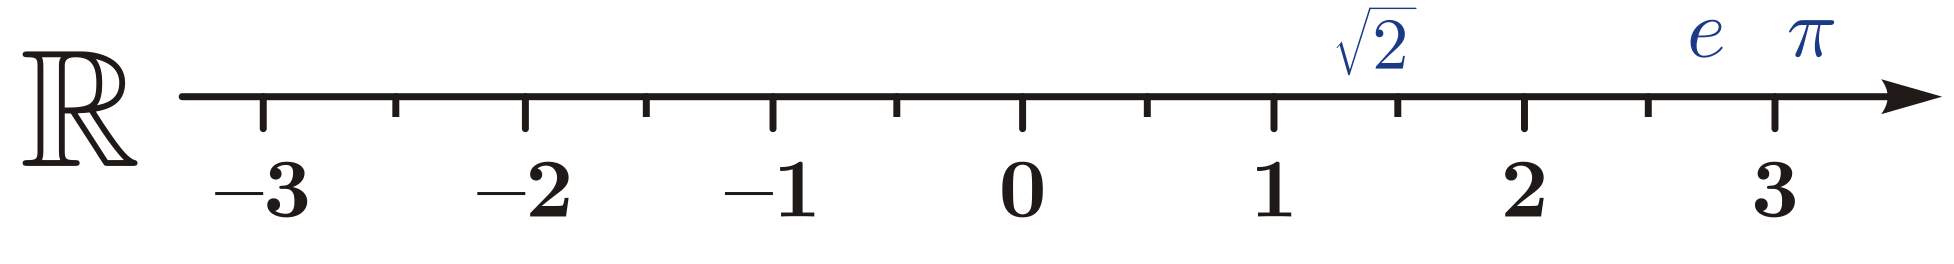
\includegraphics[scale=0.11]{images/real_line.png}. A Reta Real
\end{itemize}

Como o conjunto dos número reais pode ser descrito como pontos em uma reta numérica infinita. Se tivermos dois pontos quaisquer $a$ e $b$, de modo que $a , b \in \mathbb{R}$ e $a < b$. Temos infinitos elementos entre esses dois pontos. Por causa dessa propriedade, teremos que usar um novo símbolo para se referir aos conjuntos que são melhor descritos em termos de \textbf{intervalos} entre pontos. Abaixo coloquei uma coluna com uma representação gráfica e, ao lado, uma coluna com a respectiva definição por set builder notation.
\begin{center}
	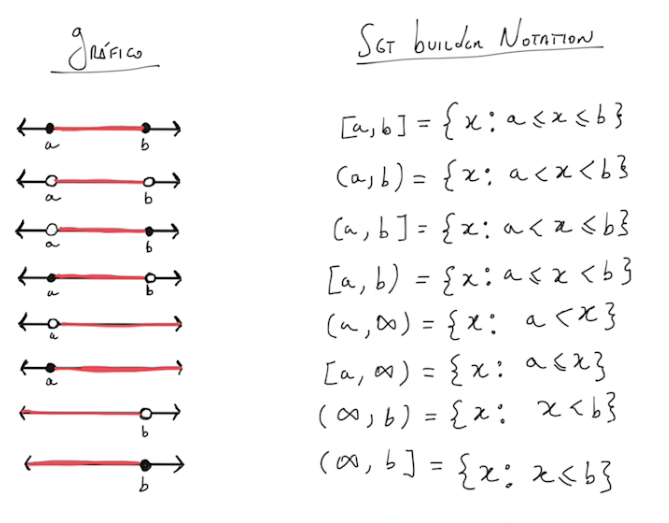
\includegraphics[scale=0.7]{images/intervals.png}
\end{center}

\section{Produto Cartesiano}
\begin{definition}[Par Ordenado]
Um \textbf{par ordenado} é uma lista\footnote{Nós definiremos uma lista no cap. 03} na forma $(x, y)$ que contém dois elementos (nesse caso, um $x$ e um $y$). Onde esses dois elementos ficam entre parênteses e separados por uma vírgula.
\end{definition}

\textbf{Regra}: Diferente dos conjuntos, a ordem dos elementos dos pares ordenados importa. Ou seja, $(x,y) \neq (y,x)$. 
\\
\\
Agora que temos a definição de par ordenado. Podemos escrever conjuntos usando esse novo conceito.

\begin{definition}[Produto Cartesiano]
O \textbf{produto cartesiano} de dois sets $A$ e $B$ é um outro set cujo símbolo é $``A \times B"$ e é definido como:
\begin{center}
$A \times B = \{ (a,b) : a \in A, b \in B \}$\footnote{Lê-se: O produto cartesiano dos conjuntos $A$ e $B$ é formado pelos pares ordenados $(a,b)$ de modo que as primeiras coordenadas são elementos de $A$ e as segundas são elementos de $B$.}
\end{center}
\end{definition}

Perceba que, se $A$ e $B$ são finitos, então $| A \times B | = |A| \ . \ |B|$. Isso é, o cardinal do produto cartesiano de dois sets é igual à multiplicação dos cardinais dos dois conjuntos.\footnote{Ao longo da etapa de Fundamentos do Projeto Matemática, faremos várias afirmações sem a devida demonstração mas, a medida que você entrar no curso de Análise, não faremos afirmações sem as devidas provas.}
\\
\\
Podemos construir um produto cartesiano onde os conjuntos $A$ e $B$ são iguais. Por exemplo: $\mathbb{R} \times \mathbb{R} = \{ (x,y) : x,y \in \mathbb{R} \}$.
\\
\\
Podemos expandir o par ordenado para infinitos elementos. Para isso vamos criar um novo conceito mais geral que abarcará o conceito de par ordenado. Chamaremos de \textbf{n-upla} a coordenada de $n$ elementos do modo $(x_1, x_2, \dots, x_n)$. Nesse conceito mais geral, um par ordenado nada mais é que uma n-upla cujo $n = 2$.
\\
\\
Para simplificar essa expressão onde temos um produto cartesiano de sets iguais, vamos criar um novo conceito que chamaremos de \textbf{potência cartesiana (Cartersian power)}. Desse modo, podemos definir o exemplo de $``\mathbb{R} \times \mathbb{R}"$ como simplesmente $``\mathbb{R}^2"$. Mais genericamente, dizemos que, para qualquer set $A$ e um $n$ positivo, o cartesian power $A^n$ será definir como:

\begin{center}
	$ A^n = \underbrace{A \times A \times ... \times A}_\text{n \ vezes} = \{ (x_1,x_2, ... , x_n) : x_1,x_2, ... , x_n \in A \} $ \footnote{Lê-se: A potência cartesiana $A^n$ é igual ao conjunto das n-uplas cujas $n$ coordenadas são elementos do conjunto $A$.}
\end{center}

\section{Subconjuntos}
Nós já aprendemos a relacionar elementos e conjuntos mas agora vamos definir um método de relacionar conjuntos entre si. A primeira relação que vamos explorar é a que expressa a situação onde todos os elementos de um conjunto também são elementos de outro conjunto.

\begin{definition}[Subconjunto]
Suponha que existam dois sets $A$ e $B$. Se todos os elementos de $A$ também forem elementos de $B$, dizemos que $A$ é um \textbf{subconjunto (subset)} de $B$. O símbolo usado para expressar essa relação é $``\subseteq"$, ou seja, $A \subseteq B$ quer dizer que $A$ é subconjunto de $B$. Caso exista um elemento de $A$ que não seja um elemento de $B$, então escrevemos que $A \nsubseteq B$.
\end{definition}

\textbf{Atenção 1}: Uma consequência direta dessa definição de subconjunto é o fato que $\emptyset \subseteq B$ para qualquer conjunto $``B"$. A demonstração dessa afirmação é simples: Suponha que exista algum conjunto $Z$ onde $\emptyset \nsubseteq Z$. Isso significaria que existe algum $x \in \emptyset$ que não é um elemento de $Z$, ou seja, $x \notin Z$. Mas, por definição, $x \notin \emptyset$, desse modo, $\emptyset \subseteq Z$.
\\
\\
\textbf{Atenção 2}: É trivial o fato que dado um conjunto qualquer $A$, todos os elementos de $A$ pertencem a ele mesmo. Isso implica que $A \subseteq A$. Portanto, todo conjunto é subconjunto de si mesmo.
\\
\\
\textbf{Atenção 3}: Como vimos antes: $\emptyset \subseteq B$, para qualquer set B. Acontece que também é verdadeiro o fato que $\emptyset \subseteq \emptyset$. Uma vez que, se $\emptyset \nsubseteq \emptyset$ existiria algum $x$ de modo que $x \in \emptyset$ e $x \notin \emptyset$. O que é uma clara contradição.

\section{Conjunto de Partes}
\begin{definition}[Conjunto de Partes]
Dado um set qualquer $B$, o seu \textbf{conjunto de partes} ou \textbf{power set} será outro set escrito como $\mathscr{P}(B)$ e definido como:
\begin{center}
	$\mathscr{P}(B) = \{ X : X \subseteq B \}$
\end{center}
\end{definition}

\textbf{Dica}: Tem bastante informação interessante no livro. Como esse aqui é só um resumo, não vou entrar muito além da definição. Mas recomendo a leitura do material original.

\section{União, Intersecção e Diferença}
Já vimos como podemos relacionar conjuntos por \textbf{produto cartesiano} para gerar outros conjuntos. Agora vamos expandir ainda mais nosso ferramental de operações entre conjuntos.

\begin{definition}[União]
Dados dois conjuntos $F$ e $G$. A \textbf{união} entre eles será um novo set denotado por $``F \cup G"$ e definido como:
\begin{center}
	$F \cup G = \{ x : x \in F \ ou \ x \in G \}$
\end{center}
\end{definition}

\begin{definition}[Intersecção]
Dados dois conjuntos $F$ e $G$. A \textbf{intersecção} entre eles será um novo set denotado por $``F \cap G"$ e definido como:
\begin{center}
	$F \cap G = \{ x : x \in F \ e \ x \in G \}$
\end{center}
\end{definition}

\begin{definition}[Diferença]
Dados dois conjuntos $F$ e $G$. A \textbf{diferença} entre eles será um novo set denotado por $``F - G"$ e definido como:
\begin{center}
	$F - G = \{ x : x \in F \ e \ x \notin G \}$
\end{center}
\end{definition}

\textbf{Dica}: Esses conceitos são muito importantes. Mas pro curso não ficar muito grande, vou me manter só nos conceitos também. Vá ler o material original caso tenha dificuldade.

\section{Complemento}
Quando lidamos com conjuntos é comum supor que há um conjunto maior que contém todos os outros. A esse set geral chamamos de \textbf{conjunto universo} ou \textbf{conjunto universal}.

\begin{definition}[Complemento]
Dado um conjunto qualquer $H$ e o seu conjunto universo $U$. O \textbf{complemento} de $H$ é um novo set denotado por $``\overline{H}"$ e definido por:
\begin{center}
	$\overline{H} = U - H$
\end{center}
\end{definition}

\section{Diagramas de Venn}

Essa sessão eu pulei integralmente. Diagramas de Venn são ótimos pra se ter uma intuição sobre todos os conceitos que vimos até agora. Mas não são usados para provas matemáticas. Ainda vale a leitura do capítulo.

\section{Conjuntos Indexados}
As vezes é necessário trabalhar com uma quantidade consideravelmente grande de conjuntos. Para esses casos, usamos uma técnica de simplificação que é adicionar um índice numérico subscrito à alguma letra maiúscula. Desse modo, ao invés de trabalharmos com sets $A$, $B$ e $C$, podemos trabalhar com os sets $A_1$, $A_2$ e $A_3$.
\\
\\
Podemos relacionar esses subscritos à um outro set. O nome dado a esse set é \textbf{conjunto índice (index set)}. Nos exemplos acima, podemos dizer que todos os subscritos pertencem ao conjunto $\{ 1 , 2 , 3 \}$.
\\
\\
Agora podemos adicionar essa técnica às relações de união e intersecção entre esses conjuntos indexados para um numero arbitrariamente grande. Além disso, vamos usar uma notação similar a do somatório\footnote{\href{https://pt.khanacademy.org/math/algebra2/sequences-and-series/alg2-sigma-notation/v/sigma-notation-sum}{Link para uma aula sobre a notação Sigma.}} para definir essas relações.

\begin{definition}[União de Sets Indexados]
Dados os conjuntos $A_1$, $A_2$, $A_3$, $\dots$, $A_n$ e o index set $I = \{ 1 , 2 , \dots , n \}$, temos que
\begin{center}
	$\bigcup_{i \in I}\limits = \{ x : x \in A_i \ para \ algum \ A_i, \ onde \  i \in I \}$
\end{center}
\end{definition}

\begin{definition}[Intersecção de Sets Indexados]
Dados os conjuntos $A_1$, $A_2$, $A_3$, $\dots$, $A_n$ e o index set $I = \{ 1 , 2 , \dots , n \}$, temos que
\begin{center}
	$\bigcap_{i \in I}\limits = \{ x : x \in A_i \ para \ todo \ A_i, \ onde \  i \in I \}$
\end{center}
\end{definition}

O livro tem dois exemplos bem interessantes da aplicação dos conceitos que acabamos de definir. A essa altura você deve conseguir entender os dois.

\section{Conjuntos que são Sistemas Numéricos}

A maioria dos conjuntos que trabalhamos são conjuntos que possuem estruturas e propriedades especiais. No caso dos conjuntos numéricos tomamos como certo que os seus elementos podem ser somados, multiplicados e possuem relações que obedecem as regras que passamos todo o ensino infantil, fundamental e médio aprendendo e aplicando. Como esse livro é introdutório, todas essas características clássicas dos sistemas numéricos serão tomadas como verdade. Mas saiba que as relações que achamos ser naturais possuem comprovações bastante complexas que você pode procurar por conta própria.
\\
\\
Aqui o autor elenca algumas propriedades que tomaremos como verdades sem que sejam devidamente definidas e demonstradas:
\begin{itemize}
	\item Propriedade Comutativa/Associativa/Distributiva da Adição/Subtração/Multiplicação/Divisão
	\item Ordenação Natural dos elementos numéricos de $\mathbb{R}$
	\item Os subconjuntos de $\mathbb{N}$ obedecem ao \href{https://pt.wikipedia.org/wiki/Princ%C3%ADpio_da_boa_ordena%C3%A7%C3%A3o}{Princípio da Boa Ordenação}.
\end{itemize}

\textbf{Comentário}: Agora a gente vai adentrar um pouco nas propriedades que podemos derivar desses pressupostos acima. Pode parecer que é um papo chato, mas a sua missão é se certificar que você é capaz de compreender toda a explicação. Vença a preguiça.
\\
\\
Uma conclusão que podemos tirar do princípio da boa ordenação é que dado um conjunto não nulo qualquer $A \subseteq \mathbb{N}$ sempre vai haver um $x_0 \in A$ que seja o seu \textbf{menor elemento}. De modo parecido, para qualquer $b \in \mathbb{Z}$, qualquer conjunto não nulo $A \subseteq \{ b, b+1, b+2, b+3, \dots \}$ também possui um \textbf{menor elemento}.

\begin{fact}[Division Algorithm]
Dados dois inteiros $a$ e $b$, onde $b > 0$. Existem outros dois inteiros únicos $q$ e $r$ para qual $a = qb + r$ e $0 \leq r < b$.
\end{fact}

Agora o autor demonstra a existência de $r$ e $q$ com suas propriedades. Mas a gente pretende estender a prova para a unicidade\footnote{Eu achei um esboço de demonstração em JOHNSTON, William; MCALLISTER, Alex. A transition to advanced mathematics: a survey course. OUP USA, 2009. p. 97.} desses valores.

\begin{demonstration}[\small Division Algorithm - Existência de $r$ e $q$]
Dados $a,b \in \mathbb{Z}$ e $b > 0$, é possível criar um set do tipo:
\begin{center}
	$ A = \{ a - xb : x \in \mathbb{Z}, 0 \leq a - xb \} \subseteq \mathbb{N}^0 $
\end{center}
Desse modo, $A \subseteq \mathbb{N}^0$. Por causa disso, podemos aplicar o princípio da boa ordenação em $A$ e dizer que existe algum elemento $r$ que seja o menor elemento de $A$.
\\
\\
Como $r \in A$ ele pode ser escrito da forma $r = a - qb$ onde $x = q \in \mathbb{Z}$. Desse fato podemos tirar duas informações úteis: 1) $a = r + qb$ e 2) Como $r \in \mathbb{N}^0$, então $r \geq 0$.
\\
\\
Agora só nos resta provar que $r < b$ mas para isso, vamos usar o pensamento contrário: O que aconteceria se $r \geq b$?
\\
\\
Ora, se $r \geq b$, então a subtração $r - b$ será um número positivo, portanto será também um elemento de $\mathbb{N}^0$. Podemos reescrever essa subtração como $r - b = (a - qb) - b = a - (q + 1)b$. 
\\
\\
Mas veja só que estranho, $q + 1$ certamente será um elemento de $\mathbb{Z}$. Logo, o número expresso por $a - (q + 1)b$ também será um elemento de $A$ (nesse caso, $(q + 1)$ é o $x$). Portanto, não é possível que $r$ seja o seu menor elemento visto que $r - b$ também é um elemento de $A$ e é menor que $r$. Isso é uma clara contradição. Isso é justamente isso que queríamos mostrar: Quando tomamos $r \geq b$ acabamos com uma contradição\footnote{O nome dessa técnica é prova por contradição. Falaremos dela mais pra frente no curso.}, portanto, só podemos aceitar o oposto, ou seja, sabemos que $r < b$. Com isso finalizamos a demonstração da existência de $r$ e $q$. $\ \blacksquare$ \footnote{Esse quadrado preto é usado para pontuar o final de uma demonstração.}
\end{demonstration}


\section{O Paradoxo de Russell}

Até agora trabalhos a distinção entre "elementos" e "conjuntos". Mas, na verdade, qualquer número (ou seja, elemento de sets numéricos) pode, sim, ser interpretado como um conjunto.\footnote{Existe um mundo de teoria sobre conjuntos, nós não temos tempo pra entrar muito fundo nessa questão. Então vá atrás de livros sobre teoria dos conjuntos e seja feliz.}. Até mesmos as operações matemáticas podem ser definidas usando-se teoria dos conjuntos. O Autor vai até mais longe "Qualquer entidade matemática é um conjunto, mesmo que não escolhamos pensar desse modo".
\\
\\
Essa parte do paradoxo de Russell não serve pro resto do livro mas é bem legal de saber. O que Bertrand Russell propôs foi o seguinte conjunto:
\begin{center}
	$ A = \{ X : X $ é um set e $X \notin X \}$\footnote{Ou seja, A é formado por todos os conjuntos que não possuem a si mesmo como elemento.}
\end{center}
E perguntou: "O conjunto $A$ é um elemento de si mesmo?".
\\
\\
Acredite, apenas esse enunciado foi uma baita dor de cabeça para os matemáticos na época. Esse assunto não é necessário para a compreensão do resto desse material. Se você quiser entender um pouco mais, confira esse \href{https://www.youtube.com/watch?v=AQTTYAM8BF0}{link} ou esse \href{https://www.youtube.com/watch?v=0Bs0lJRxOaI}{link}, ou ainda esse último \href{https://www.youtube.com/watch?v=HeQX2HjkcNo}{link}.
\\
\\
\textbf{Dica}: Vai ler o livro nessa parte. O professor explica bem melhor sobre o paradoxo.

%%%%%%%%%%%%%%%%%%%%%%%% CHAPTER %%%%%%%%%%%%%%%%%%%%%%%%
\chapter{Lógica}

\begin{chapquote}{página 34}
	``Logic is a systematic way of thinking that allow us to parse the meanings of sentences and to deduce new information from old information. [...] Logic is  a process of deducing information correctly, not just deducing correct information''
\end{chapquote}

\section{Proposições}

O estudo da lógica começa com as proposições. Uma \textbf{proposição} é uma sentença ou expressão matemática que seja definitivamente verdadeira ou falsa. Em cima dessas proposições é que aplicamos a lógica para produção de novas proposições. Qualquer resultado ou teorema provado é, na verdade, uma proposição\footnote{Isso inclui o teorema de Pitágoras, por exemplo.}. 
\\
\\
\textbf{Aviso}: Ao longo desse capítulo a palavra "proposição" \ vai ser repetida muitas vezes. Essa repetição é proposital. Eu quero que você internalize a importância desse conceito para a análise matemática.
\\
\\
Podemos usar letras para nomear proposições. Por exemplo, a proposição "Se um número $x$ é múltiplo de 6, então $x$ é par" \  pode ser resumida em uma letra. Nesse caso diremos que "$P$" \ é a proposição acima. Dessa feita, sempre que dissermos $P$ é falso ou $P$ é verdadeiro, estamos nos referindo a proposição completa.
\\
\\
Quando uma proposição possuir variáveis, podemos escreve-la de uma maneira similar às funções. No exemplo do parágrafo acima, podemos usar o símbolo $P(x)$ para expressar que a proposição $P$ possui uma variável $x$ dentro dela.\footnote{Fique atento para não confundir quando estivermos nos referindo a funções e proposições.}
\\
\\
Uma \textbf{sentença aberta} é uma proposição cuja validade depende da sua variável. Ou seja, dependendo do valor que você der para a variável, a proposição pode ser verdadeira ou falsa.
\\
\\
Esse livro do professor Hammack é justamente sobre o método de como se provar que uma proposição é verdade ou falsa. Existem estratégias de raciocínio que podem ser usadas para demonstrar proposições e, consequentemente, teoremas complexos. Nosso objetivo nesse curso é lhe ensinar essas técnicas.

\section{Operadores: e, ou, não}

Até agora foi dito que você pode usar proposições junto à lógica para se chegar a outras proposições. Então vamos aprender como trabalhar com mais de uma proposição por meio dos \textbf{operadores lógicos}.
\\
\\
O primeiro operador que vamos aprender é o "$e$". Dadas as proposições $P$ e $Q$. Podemos criar uma nova proposição através desse operador. Quando escrevemos $R: P \ e \ Q$, estamos criando uma nova proposição $R$ que é composta de das duas proposições $P$ e $Q$. O símbolo usado para esse conectivo é o "$\land$". Aqui em baixo vamos colocar a tabela verdade\footnote{Se você não sabe o que são tabelas-verdades então dá uma lida nesse \href{https://www.youtube.com/watch?v=hWEZsyF3ZZc}{link}.} desse operador\footnote{"V" \ significa Verdadeiro e "F" \  significa Falso.}.

\begin{center}
\begin{tabular}{| c c || c | }
\hline
 P & Q & $P \land Q$ \\ 
 \hline
 V & V & V \\  
 V & F & F \\  
 F & V & F \\  
 F & F & F \\
 \hline
\end{tabular}
\end{center}

Outro operador lógico clássico é o "ou". O símbolo dele é o "$\lor$". Eu sei, parece muito com o símbolo do "e" \ mas a  gente não pode fazer nada a não ser decorar bem a distinção entre esses dois símbolos. A tabela-verdade do "ou" \ segue abaixo.

\begin{center}
\begin{tabular}{ | c c || c | }
\hline
 P & Q & $P \lor Q$ \\ 
 \hline
 V & V & V \\  
 V & F & V \\  
 F & V & V \\  
 F & F & F \\
 \hline
\end{tabular}
\end{center}

\textbf{Atenção}: O significado da palavra "ou" \ na linguagem do dia a dia é diferente do significado empregado no contexto da lógica. Quando usamos o conectivo "ou" \ na lógica, fica implícita a possibilidade de ambas as proposições sejam verdadeiras ao mesmo tempo. Para as situações onde queremos que apenas uma proposição seja aceita mas não ambas, usamos um "ou exclusivo"\footnote{O símbolo desse é o "$\oplus$".} \ dos seguintes modos: 

\begin{itemize}
\item ou $P$ ou $Q$
\item $P$ ou $Q$, mas não ambos
\item Exatamente um de $P$ ou $Q$
\end{itemize}

O último operador que veremos é a \textbf{negação}. Ela inverte a condição da proposição onde é aplicada. Seu símbolo é o "$\sim$"\footnote{Existem outras representações desse operador: $\lnot$ , $\veebar$ , $\dot\lor$}, ou seja, se uma proposição é verdadeira, ao aplicarmos a negação à ela, tornamos essa proposição falsa. A tabela-verdade desse operador é bem simples.

\begin{center}
\begin{tabular}{ | c || c | }
\hline
 P & $\sim P$ \\ 
 \hline
 V & F \\  
 F & V \\
 \hline
\end{tabular}
\end{center}

\section{Proposições Condicionais}

Podemos ainda combinar proposições de outra maneira. Sejam as proposições $P$ e $Q$. Podemos dizer que "Se $P$ for verdade, então $Q$ também será verdadeiro". O símbolo usado para esse conectivo se...então é o "$\implies$". Uma proposição desse tipo é chamada de \textbf{proposição condicional}. Leia a página 43 do livro caso você esteja com dúvida sobre as últimas duas linhas da tabela-verdade.\footnote{O autor dá a dica de você pensar nas proposições compostas como promessas feita por alguém. Isso ajuda muito a entender como as tabelas-verdade são construídas.}

\begin{center}
\begin{tabular}{ | c c || c | }
\hline
 P & Q & $P \implies Q$ \\ 
 \hline
 V & V & V \\  
 V & F & F \\  
 F & V & V \\  
 F & F & V \\
 \hline
\end{tabular}
\end{center}

\textbf{Dica}: Nessa parte do livro o professor coloca bastante esforço em explicar esse conceito. Se você não conseguir entender essa tabela-verdade acima, recomendo dar uma lida seção que começa na página 42.

\section{Proposições Bicondicionais}

Existem situações onde duas proposições são mutuamente condicionais, ou seja, $P \implies Q$ e $Q \implies P$. Nesses casos usamos o conectivo "se e somente se" cujo símbolo é "$\iff$".  A tabela-verdade segue abaixo.

\begin{center}
\begin{tabular}{ | c c || c | }
\hline
 P & Q & $P \iff Q$ \\ 
 \hline
 V & V & V \\  
 V & F & F \\  
 F & V & F \\  
 F & F & V \\
 \hline
\end{tabular}
\end{center}

\textbf{Desafio}: Na prática, a proposição bicondicional $P \iff Q$ nada mais é do que a proposição composta $(P \implies Q) \land (Q \implies P)$. Leia a seção 2.5 e volte aqui. Seu desafio é provar essa equivalência.\footnote{Posta uma foto da tabela-verdade composta e me marca no  \href{https://twitter.com/bruno_ruas2}{twitter}.}.


\section{Tabelas-Verdade para Proposições}

Agora que você sabe as tabelas-verdade de $\land$,$\lor$,$\sim$,$\implies$ e $\iff$, você deve internalizá-las de modo a serem muito naturais ao avaliar a validade de uma proposição cuja construção utilize esses operadores.
\\
\\
Vamos trabalhar uma proposição composta que expressa a seguinte situação: Dadas duas proposições $P$ e $Q$, somente uma delas é verdadeira mas não ambas. Não existe um operador que nos permita construir uma proposição apenas com um único símbolo. Para podermos construir tal proposição temos que combinar nossos operadores do seguinte modo:

\begin{center}
	$(P \lor Q) \ \land \ \sim (P \land Q)$
\end{center}

Essa proposição pode assustar numa primeira olhada, contudo, ela expressa exatamente nossa intenção anteriormente explicitada. Podemos resumi-la como: "$P$ ou $Q$ são verdadeiras, mas não é o caso onde $P$ e $Q$ são verdadeiras.
\\
\\
A tabela-verdade dessa proposição é a seguinte:

\begin{center}
\begin{tabular}{ | c c || c c || c || c | }
\hline
 P & Q & $(P \lor Q)$ & $(P \land Q)$ & $\sim (P \land Q)$ & $(P \lor Q) \ \land \ \sim (P \land Q)$\\
 \hline
 V & V & V & V & F & F \\  
 V & F & V & F & V & V \\  
 F & V & V & F & V & V \\  
 F & F & F & F & V & F \\
 \hline
\end{tabular}
\end{center}

Calma. É bem mais tranquilo do que parece. Vamos analisar essa tabela por partes. Nas primeiras duas colunas temos as proposições iniciais $P$ e $Q$. Nas linhas estão as situações onde testamos o que acontece quando elas são verdadeiras ou falsas. Na segunda parte temos as proposições compostas por $\lor$ e $\land$ (que você já conhece a tabela-verdade). Na parte 3 temos apenas a negação da coluna $(P \land Q)$. Se criarmos mais duas proposições do tipo $Z : (P \lor Q)$ e $W : \  \sim(P \land Q)$. Podemos reduzir a última coluna como a tabela-verdade abaixo:

\begin{center}
\begin{tabular}{ | c c || c c || c | }
\hline
 P & Q & Z & W & $Z \land W$ \\ 
 \hline
 V & V & V & F & F \\  
 V & F & V & V & V \\  
 F & V & V & V & V \\  
 F & F & F & V & F \\
 \hline
\end{tabular}
\end{center}

Que é exatamente igual à última coluna da tabela-verdade anterior. Portanto, nossa proposição é verdadeira exatamente quando $P$ ou $Q$ são verdadeiros mas não quando ambos são verdadeiros. Parabéns por ter entendido até aqui!
\\
\\
\textbf{Comentário}: Eu peguei esse exemplo direto do livro. Contudo, eu pensei um pouco e uma equivalência a essa proposição composta (bem mais simples) seria $\sim(P \iff Q)$\footnote{Você consegue ver isso?}.

\section{Equivalência Lógica}

Nesse meu comentário acima já vemos um exemplo de equivalência lógica. Quando temos tabelas-verdade iguais para proposições diferentes. Podemos dizer que elas são \textbf{logicamente equivalentes}.
\\
\\
Esse conceito é importante porque podemos trabalhar o mesmo problema de diferentes abordagens e acabarmos chegando no mesmo resultado. Cada abordagem pode ter facilidades que queiramos explorar e que vão nos permitindo desenrolar o pensamento necessário para uma demonstração mais complexa.
\\
\\
Muitos teoremas matemáticos usam a forma $P \implies Q$. Mas, não raramente, precisamos usar a equivalência lógica e trabalhar com a proposição $\sim (Q) \implies \sim (P)$. Para ver essa equivalência, basta construir as tabelas-verdade das duas proposições.\footnote{Fica como dever de casa pra você.}
\\
\\
Existem equivalências que são tão importantes que possuem um nome particular. As duas abaixo são chamadas de Lei de DeMorgan.

\begin{center}
$\sim(P \land Q) = (\sim P) \lor (\sim Q)$ \\
$\sim(P \lor Q) = (\sim P) \land (\sim Q)$
\end{center}

A tabela-verdade da primeira parte é:
\begin{center}
\begin{tabular}{ | c c || c c c || c c | }
\hline
P & Q & $\sim P$ & $\sim Q$ & $P \land Q$ & $\sim (P \land Q)$ & $(\sim P) \lor (\sim Q)$ \\
\hline
V & V & F & F & V & F & F \\
V & F & F & V & F & V & V \\
F & V & V & F & F & V & V \\
F & F & V & V & F & V & V \\
\hline
\end{tabular}
\end{center}

A tabela-verdade da segunda parte é:
\begin{center}
\begin{tabular}{ | c c || c c c || c c | }
\hline
P & Q & $\sim P$ & $\sim Q$ & $P \lor Q$ & $\sim (P \lor Q)$ & $(\sim P) \land (\sim Q)$ \\
\hline
V & V & F & F & V & F & F \\
V & F & F & V & V & F & F \\
F & V & V & F & V & F & F \\
F & F & V & V & F & V & V \\
\hline
\end{tabular}
\end{center}

Nessa parte o professor elenca várias equivalências que podem ser verificadas por suas respectivas tabelas-verdade.

\begin{itemize}
\item $ P \implies Q = (\sim Q) \implies (\sim P) $ - Lei Contrapositiva
\item $ \sim (P \land Q) = \  (\sim P) \ \lor \ (\sim Q) $ - Lei de DeMorgan 1
\item $ \sim (P \lor Q) = \  (\sim P) \ \land \ (\sim Q) $ - Lei de DeMorgan 2
\item $ P \land Q = Q \land P $ - Lei Comutativa 1
\item $ P \lor Q = Q \lor P $ - Lei Comutativa 2
\item $ P \land (Q \lor R) = (P \land Q) \lor (P \land R)$ - Lei Distributiva 1
\item $ P \lor (Q \land R) = (P \lor Q) \land (P \lor R) $ - Lei Distributiva 2
\item $ P \land (Q \land R) = (P \land Q) \land R $ - Lei Associativa 1
\item $ P \lor (Q \lor R) = (P \lor Q) \lor R $ - Lei Associativa 2
\end{itemize}

\textbf{Comentário}: Como são muitas equivalências, se eu colocar todas as tabelas-verdade aqui vai ficar uma poluição muito grande. Então cabe a você demonstrar todas essas equivalências por conta própria. Não confie só porque está escrito ai. Demonstre com seu próprio esforço todas elas.

\section{Quantificadores}

Até agora nós já vimos um punhado de símbolos que nos permitem construir proposições consideravelmente complexas, bem como, achar as equivalências entre diferentes proposições. Mas ainda temos um problema para superar: o que fazer quando temos que lidar com infinitos elementos?
\\
\\
O professor usa o seguinte exemplo: Imagine um conjunto infinito de números inteiros $X = \{ x_1,x_2,x_3, \dots \}$. Com os símbolos apresentados até agora, como faríamos para representar as seguintes proposições?

\begin{itemize}
\item $Z_1:$ "Todos os elementos de $X$ são ímpares"
\item $Z_2:$ "Pelo menos um elemento de $X$ é ímpar"
\end{itemize}

Primeiro vamos definir a proposição $P :$ "O número $x$ é ímpar". Para a primeira proposição ($Z_1$), teríamos algo parecido com 

$$P(x_1) \land P(x_2) \land P(x_3) \land \dots$$

E para a segunda proposição ($Z_2$), algo como

$$P(x_1) \lor P(x_2) \lor P(x_3) \lor \dots$$

Ou seja, acabaríamos com proposições de tamanho infinito.
\\
\\
Para superar essa dificuldade, vamos introduzir novos símbolos "$\forall$" \ e "$\exists$". O símbolo $\forall$ significa "para todos" \ e o símbolo $\exists$ significa "existe algum". Desse modo podemos reescrever as proposições anteriores como:

\begin{itemize}
\item $Z_1: \forall \ x \in X, P(x)$
\item $Z_2: \exists \ x \in X, P(x)$
\end{itemize}

Nós chamamos esses novos símbolos de \textbf{quantificadores}.\footnote{Não sei você, mas pra mim esse daria um bom nome de banda.} Esse nome é porque eles se referem a alguma propriedade da quantidade de algo. $\forall$ é chamado de \textbf{quantificador universal} e $\exists$ é chamado de \textbf{quantificador existencial}. Proposições que contenham esses símbolos são chamadas de \textbf{proposições quantificadas}.
\\
\\
\textbf{Dica}: Leia o exemplo 2.5 do livro. O professor Hammack dá 4 exemplos em inglês e "traduz" \ esses exemplos para os símbolos que já aprendemos até agora.

\section{Um pouco mais de Proposições Condicionais}

Na seção 2.1 nós vimos que uma \textbf{sentença aberta} é uma proposição cuja validade depende do valor da variável. Contudo, uma característica que os quantificadores possuem é transformar sentenças abertas em proposições.
\\
\\
Dada a sentença aberta "$x$ é par $\implies$ $x$ é múltiplo de 6". A validade dessa afirmação depende totalmente do valor dado para a variável $x$. Agora, quando adicionamos um quantificador "$\forall \ x \in \mathbb{Z}, x$ é par $\implies x$ é múltiplo de 6", ela se torna uma proposição, ou seja, podemos definir se ela é verdadeira ou falsa (nesse caso, falsa).
\\
\\
De maneira geral, dadas duas proposições $Q(x)$ e $P(x)$, a expressão $\forall \ x \in \mathbb{Z}, P(x) \implies Q(x)$ é verdadeira ou falsa. Logo, ela é uma proposição e não uma sentença aberta.
\\
\\
Agora chegamos no ponto importante sobre esse assunto: sempre que você ver duas proposições a respeito de uma variável que seja elemento de algum conjunto (previamente definido), uma expressão da forma $P(x) \implies Q(x)$ deve ser interpretada como sendo uma proposição do tipo $\forall \ x \in Conjunto, P(x) \implies Q(x)$. Ou seja, se uma proposição condicional não estiver quantificada explicitamente, então existe um quantificador implícito atrelado a ela. O motivo desse quantificador não aparecer é que cansa ter que ficar escrevendo toda hora "$\forall \ x \in Conjunto$".
\\
\\
Agora nós vamos definir de maneira mais geral (mas consistente com o que foi dito na seção 2.1) as proposições condicionais.

\begin{definition}[Proposição Condicional]
Se $P$ e $Q$ são proposições ou sentenças abertas, então "Se $P$, então $Q$" \  será uma proposição.\\
Essa proposição será verdadeira se for impossível que $P$ seja verdadeira enquanto $Q$ seja falsa. E será falsa se existir alguma situação onde $P$ é verdadeira e $Q$ é falsa.
\end{definition}

\section{Traduzindo Português para Lógica Simbólica}

Quando estamos lendo provas de teoremas, sempre devemos estar atentos para a estrutura lógica e o significado das sentenças. Não é raro ter que converter as expressões feitas de palavras para expressões feitas dos símbolos que estudamos até agora. Essa seção é uma prática para você exercitar essa competência.
\\
\\
\textbf{Comentário}: A partir desse ponto pode ser que você veja alguns conceitos que não foram previamente explicados no material. Não se assuste por causa disso. Foque apenas na lógica e no que você aprendeu até aqui.
\\
\\
\textbf{Exemplo 1}: O teorema do valor médio do Cálculo Infinitesimal.
\\
\hrule
\vspace{5pt}
Se $f$ é contínua no intervalo $[a,b]$ e diferenciável em $(a,b)$, então existe um número $c \in (a,b)$ onde $f'(c) = \dfrac{f(b) - f(a)}{b - a}$.
\vspace{5pt}
\hrule
\vspace{5pt}
A tradução para a forma simbólica dessa afirmação é:
$$ \left( (f \ cont. \ em \  [a,b]) \land (f \ dif. \ em \  (a,b)) \right) \implies \left(\exists \ c \in (a,b), f'(c) = \dfrac{f(b) - f(a)}{b - a} \right) $$

Eu sei, ficou meio poluído. Pra melhorar um pouco vamos definir novas proposições e limpar um pouco essa sujeira toda. $P : $"$f$ é contínua no intervalo $[a,b]$", $Q : $"$f$ é diferenciável em $(a,b)$".

$$ \left( P \land Q \right) \implies \left(\exists \ c \in (a,b), f'(c) = \dfrac{f(b) - f(a)}{b - a} \right) $$
\\
\\
\textbf{Exemplo 2}: A conjectura de Goldbach.
\\
\hrule
\vspace{5pt}
Todo número inteiro par maior que $2$ é a soma de dois primos.
\vspace{5pt}
\hrule
\vspace{5pt}
A tradução para a forma simbólica dessa afirmação é:
$$ \left( n \in X \right) \implies \left( \exists \ p,q \in P, n = p + q \right) $$
Ou então, podemos usar essa outra forma equivalente:
$$ \forall \ n \in X, \exists \ p,q \in P, n = p + q $$
\\
Sendo $P = \{x : x \ é \ primo \}$ e $X = \{ 4,6,8,10.\dots \}$. 
\\
\\
Esse exemplo acima nos mostra uma relação interessante entre as proposições do tipo $(n \in X) \implies Q(n)$ e as do tipo $\forall \ n \in X, Q(x)$. Toda proposição universalmente quantificada\footnote{Ou seja, com o uso do $\forall$.} pode ser expressa como uma proposição condicional.


\begin{fact}[Equivalência de proposições]
Suponha que $X$ é um conjunto e $Q(x)$ é uma proposição a respeito de cada $x \in X$. As proposições abaixo são equivalentes:
$$ \forall \ x \in X, Q(x) $$
$$ (x \in X) \implies Q(x) $$
\end{fact}

Essas equivalências são importantes porque podemos trocar a maneira como um teorema se apresenta na hora de tentar provar ou desprovar uma proposição.
\\
\\
\textbf{Aviso}: Na hora que você ler um teorema, evite ir direto para as palavras "ou", "se", "e" \ como se elas sempre significassem os seus respectivos valores lógicos. O contexto é quem diz o real significado das palavras. Sempre analise o enunciado inteiro antes de transcrever para a linguagem simbólica da lógica.

\section{Negando Proposições}

Não é raro que ao tentar demonstrar uma proposição complexa $R$, por exemplo, seja mais fácil trabalhar com a negação dessa proposição $\sim R$. Mas na frente do curso você verá que essa é uma das técnicas usadas para provar teoremas.
\\
\\
Também não é incomum termos que lidar com negações de proposições quantificadas. Considere a proposição $\sim(\forall \ x \in \mathbb{N}, P(x))$. Podemos ler como "Não é o caso que $P(x)$ é verdade para todos os $x$ números naturais". Ou seja, a negativa dessa proposição envolve outro quantificador (o de existência). De modo que podemos reescrever essa negação como $\exists \ x \in \mathbb{N},\sim P(x)$.
\\
\\
Chegamos em um ponto importante aqui. Os quantificadores são usados para negar um ao outro. Observe as seguintes equivalências:

$$ \sim (\forall \ x \in X, P(x)) = \exists \ x \in X, \sim P(x) $$
$$ \sim (\exists \ x \in X, P(x)) = \forall \ x \in X, \sim P(x) $$

\textbf{Comentário}: Se você leu com atenção até aqui, você deve ser capaz de compreender essas equivalências. Se elas não fazem sentido na sua cabeça, me manda uma dm no \href{https://twitter.com/bruno_ruas2}{twitter} explicando qual a sua dúvida. Eu posso melhorar o texto com o seu feedback.
\\
\\
Quando se está escrevendo demonstrações, as vezes é necessário negar proposições condicionais $P \implies Q$. Se você aprendeu a tabela-verdade desse tipo de operador, você sabe que a única maneira de ele ser falso é quando temos $P$ verdadeiro e $Q$ falso. Em termo da lógica dizemos que $\sim (P \implies Q) = P \land \sim Q$. 
\\
\\
\textbf{Dica}: Tente fazer o exercício 5 da seção 2.10. Tem a solução dele no final do livro. Se mesmo assim você não conseguir entender, comenta sua dúvida na postagem dessa aula no \href{https://economiamainstream.com.br/artigo/matematica/}{Economia Mainstream}.

\section{Inferência Lógica}

A inferência lógica é o processo de se tirar conclusões dadas premissas e regras previamente estabelecidas. Existem algumas maneiras de se trabalhar esse processo de pensamento. O professor elenca 3 modos: modus ponens, modus tollens e eliminação.

\begin{align*}
Modus \ Ponens && Modus \ Tollens && Elimina\c{c}\~{a}o \\
P \implies Q & & P \implies Q     & & P \lor Q \\
P            & & \sim Q           & & \sim P   \\
\dfrac{\hspace*{50pt}}{Q}  & & \dfrac{\hspace*{50pt}}{\sim P} & & \dfrac{\hspace*{50pt}}{Q}
\end{align*}


Os diagramas acima são fáceis de se ler. Tudo que está em cima da linha é dado como verdadeiro. O que está abaixo é a consequência lógica do que está acima. É importante que você internalize esses métodos de pensamento. Você usará bastante ao longo da sua jornada pela matemática.

\section{Nota Importante}

Para finalizar, o professos elenca 3 grandes motivos para se estudar lógica: 1) As tabelas-verdade nos dizem exatamente os significados das palavras "e", "ou", "não", "se...então", etc; 2) As regras da inferência produzem um sistema onde podemos deduzir novas informações de afirmações anteriores; 3) Regras lógicas (como a lei de DeMorgan) nos ajudam a transformar proposições em formatos que sejam mais fáceis de se trabalhar e que são equivalentes.
\\
\\
Lógica é a linguagem-comum que toda a Matemática utiliza, então temos que ter uma boa base para poder escrever e entender a própria matemática. Durante o resto desse livro não usaremos com tanta frequência os símbolos que vimos $(\land, \lor, \implies, \iff, \sim, \forall, \exists)$ mas sempre que ler uma passagem matemática, você deve usa-los, mentalmente ou em papel, para se certificar que você a compreendeu de uma maneira inequívoca e verdadeira.

%%%%%%%%%%%%%%%%%%%%%%%% CHAPTER %%%%%%%%%%%%%%%%%%%%%%%%
\chapter{Contagem}


\begin{chapquote}{página 65}
	``Counting can become quite subtle, and in this chapter we explore some of its more sophisticated aspects. Our goal is still to answer the question 'How many?' but we introduce mathematical techniques that bypass the actual process of counting individual objects''
\end{chapquote}

\section{Listas}

Uma \textbf{lista} é uma sequência ordenada de objetos. Esses objetos são mantidos entre um par de parênteses e separados por vírgulas. Os objetos dentro de uma lista são chamados de \textbf{entradas}\footnote{Do original, \textbf{entries}}. Já que uma lista é uma sequência ordenada, é evidente que a ordem dos seus elementos é suficiente para distinguir listas que contenham os mesmo objetos.

$$ (a,b,c) \neq (c,b,a) $$

\textbf{Comentário}: Também é comum escrever uma lista sem os parênteses e as vírgulas. Esse formato de escrita se chama \textbf{string}. Nesse caso $(a,b,c)$ é a mesma coisa de $abc$. Essa outra maneira só é usada quando não há risco de confusão entre as entradas da lista. Fica ligado e mantém essas duas formas de escrita como padrão.
\\
\\
Como já vimos conjuntos no capítulo 01, podemos usá-los para comparação. No caso dos conjuntos a ordem dos elementos não importa na comparação. Ou seja, $\{a,b,c\} = \{c,b,a\}$. Já vimos acima que essa propriedade não é mantida nas listas. 
\\
\\
Diferentemente dos conjuntos, uma lista pode ter entradas repetidas sem nenhum problema. A lista $(a,a,a,a,b)$, por exemplo, é perfeitamente aceitável.
\\
\\
Tal qual a cardinalidade dos conjuntos, nós contamos quantas entradas existem em uma lista. Chamamos essa medida de \textbf{comprimento}. A lista $(a,a,a,a,b)$ possui um comprimento de 5.
\\
\\
\textbf{Regra}: Duas listas são \textbf{iguais} se possuírem exatamente as mesmas entradas nas mesmas posições. Ou seja, também possuem o mesmo comprimento.
\\
\\
Só existe uma lista cujo comprimento é igual a zero. Denominamos essa lista de \textbf{lista vazia}. Denotada por $()$.\footnote{Sim, lembra muito o conceito de conjunto vazio.}

\section{O Princípio da Multiplicação}

Existem muitos problemas práticos que envolvem a contagem do número possível de listas que satisfazem uma determinada condição ou propriedade. Por causa disso, vamos aprender uma maneira de trabalharmos essa questão sem precisar ficar escrevendo todas as listas possíveis antes de contar os resultados.

\begin{fact}[Princípio da Multiplicação]
Suponha que em uma lista de comprimento $n$ exista $a_1$ escolhas possíveis para a primeira entrada, $a_2$ escolhas possíveis para a segunda entrada, $a_3$ escolhas possíveis para a terceira entrada e etc. Então, o total de listas diferentes que podem ser geradas por essas entradas será igual ao produto entre $a_1 \times a_2 \times a_3 \times \dots \times a_n$. 
\end{fact}

\textbf{Dica}: Nas páginas 67 e 68 do livro, o professor coloca dois exemplos que tornarão esse conceito abaixo bem mais entendível. Se você não entender como esse fato é evidente, dá uma olhada no livro e volta aqui.
\\
\\
Embora no livro não seja dada uma demonstração desse princípio. Eu acho que podemos tentar provar que essa afirmação é verdadeira. Não se preocupe se você não conseguir entender essa demonstração agora. Volte quando estiver mais adiantado no curso e tente novamente.

\begin{demonstration}[Princípio da Multiplicação\footnote{A ideia da primeira parte da demonstração para $m \leq 2$ veio desse livro: JOHNSTON, William; MCALLISTER, Alex. A transition to advanced mathematics: a survey course. OUP USA, 2009. p. 365. Pra segunda parte, onde $m > 2$, a inspiração veio desse link do 
\href{https://math.stackexchange.com/questions/3053969/using-induction-to-prove-the-multiplication-rule}{StackExchange.}}]

Começaremos com a proposição $P(m)$: "Se existirem $m \in \mathbb{N}$ conjuntos $A_i$ com $n_i$ elementos em cada conjunto onde $i \in \{1,2,\dots,m\}$. O Cardinal do produto cartesiano de todos os $m$ conjuntos será igual à multiplicação de todos os $m$ cardinais $| A_i|$, ou seja, $ |A_1 \times A_2 \times \dots \times A_m | = \prod_{i = 1}^{m}\limits | A_i | $"\footnote{O nome desse símbolo é \href{https://en.wikipedia.org/wiki/Multiplication\#Product_of_a_sequence}{"Produtório"}}.
\\
\\
Essa proposição é equivalente ao enunciado do princípio da multiplicação.\footnote{Você consegue ver essa equivalência?}
\\
\\
Quando $m = 1$, temos apenas o conjunto $A_1$ que possui $n_1$ elementos. Portanto, o cardinal de todos os $m = 1$ conjuntos é igual ao cardinal do único conjunto ($|A_m| = |A_1|$). Com isso, vemos que $P(1)$ é verdadeira.
\\
\\
$P(2)$: "Se $A_1$ e $A_2$ são conjuntos finitos onde $A_1$ contém $n_1$ elementos e $A_2$ contém $n_2$ elementos, então, o conjunto $A_1 \times A_2$ possui $n_1 \cdot n_2$ elementos".
\\
\\
A demonstração dessa proposição é simples. Para cada um dos $n_1$ elementos $a \in A_1$ na primeira coordenada do par ordenado $(a,b) \in A_1 \times A_2$, existem exatamente $n_2$ elementos $b \in A_2$. Uma vez que existem $n_1$ elementos em $A_1$ que podem ser essa primeira coordenada do par ordenado $(a,b)$, então, existem ao todo $n_1 \cdot n_2$ possíveis pares ordenados no produto cartesiano $A_1 \times A_2$.
\\
\\
Agora vamos fazer uma pequena adaptação nessa demonstração para qualquer quantidade de conjuntos, ou seja, para qualquer $P(m)$ cujo $m > 2$.
\\
\\
Suponha que agora temos 3 conjuntos: $A_1$, $A_2$ e $A_3$. Para podermos demonstrar $P(3)$: "Se $A_1 \times A_2 \times A_3$, então o cardinal será  $n_1 \cdot n_2 \cdot n_3$"\  só precisamos da seguinte linha de pensamento: Podemos definir um novo conjunto $B = A_1 \times A_2$. Desse modo, podemos reescrever o cardinal anterior como $B \times A_3$. Essa nova reescrita possui apenas dois elementos. Portanto, podemos usar a proposição já demonstrada $P(2)$ sem nenhum prejuízo.
\\
\\
Aplicando esse mesmo procedimento para qualquer $m > 2$ fica demonstrado que o cardinal de quaisquer conjuntos $A_i$ para qualquer $i \in \{1,2,\dots,m\}$ será a multiplicação do cardinal dos conjuntos $A_i$. Aplicando a equivalência da proposição $P(m)$ com o princípio da multiplicação, finalizamos a demonstração. $\blacksquare$
\end{demonstration}

Existem dois tipos de problemas que envolvem contagem de listas: Problemas que possuem entradas repetidas e Problemas que não permitem entradas repetidas. Nós podemos chamar as listas do segundo tipo de problema de \textbf{listas não repetitivas}.
\\
\\
Usando o princípio da multiplicação você é capaz de resolver todos os problemas envolvendo contagens de listas sem precisar ficar escrevendo as soluções possíveis, ao invés disso, você só precisa interpretar as opções de entradas na lista e usar a multiplicação.
\\
\\
\textbf{Dica}: Tente fazer os exemplos 3.1, 3.2 e 3.3 da página 69 até a 72.

\section{Os Princípios da Adição e Subtração}

Vamos ver mais dois princípios de contagem. Você já está familiarizado com eles mas agora definiremos esses princípios usando a linguagem dos conjuntos.

\begin{fact}[Princípio da Adição]
Suponha que um conjunto finito $X$ pode ser decomposto na união $X = \bigcup_{i = 1}^{n}\limits X_i$ onde $ X_i \cap X_j = \emptyset \ \forall \ i \neq j$. Então, $|X| = \sum_{i = 1}^{n}\limits |X_i|$.
\end{fact}

Calma. Não é difícil de entender. O que estamos dizendo ai é: "Se $X$ é um conjunto formado por $n$ outros conjuntos menores de modo que nenhum desses conjuntos possui interseção entre si. Então, o cardinal de $X$ será a soma dos cardinais de todos os $n$ subconjuntos. A única novidade nessa notação é o sigma para denominar somatório.\footnote{Já vimos essa notação no capítulo 01.}
\\
\\
\textbf{Dica}: Veja os exemplos 3.5 e 3.6 na página 75 para ter uma ideia da aplicação desses conceitos na prática.
\\
\\
Agora vamos ver o princípio da subtração. Você não deve ter grandes dificuldades de entender esse conceito.

\begin{fact}[Princípio da Subtração]
Se $X$ é um subconjunto de um conjunto finito $U$, então $|\overline{X}| = |U| - |X|$. Ou seja, se $X \subseteq U$, então $|U - X| = |U| - |X|$.
\end{fact}

Existem situações onde é mais fácil contar o total de um conjunto maior, e retirar uma parte desse total que não queremos, do que contar diretamente a parte desejada. Eu sei, tá um pouco confuso. Mas a ideia é simples: Usamos esse método para computar o que sobra após a retirada de algumas opções.

\textbf{Dica}: Dá uma lida no exemplo 3.7 novamente. A gente usa exatamente essa abordagem pra chegar no resultado.

\section{Fatoriais e Permutações}
O processo de contagem para listas não repetitivas de tamanho $n$ é tão comum que criamos um conceito especial para lidar com esse tipo de problema. O conceito em questão é o \textbf{Fatorial} ($n!$). Antes de formalizarmos o que é o fatorial, observe o quadro abaixo.
\\
\\
\begin{center}
\begin{tabular}{ | c | c | c | c | }
 \hline
 n & Elementos & Listas não repetidas de tamanho $n$ & $n!$ \\ 
 \hline
 0 & $\{\}$ & $()$ & 1 \\
 1 & $\{a\}$ & $(a)$ & 1 \\
 2 & $\{a,b\}$ & $(a,b), (b,a)$ & 2 \\
 3 & $\{a,b,c\}$ & $(a,b,c),(a,c,b),(b,a,c),(b,c,a),(c,a,b),(c,b,a) $ & 6 \\
 \vdots & \vdots & \vdots & \vdots \\
\end{tabular}
\end{center}

Consegue ver como a quantidade de listas não repetitivas cresce rápido com apenas o incremento de 1 elemento no exemplo?. O número da última coluna é obtido pela aplicação do princípio da multiplicação. Nós chamamos esse número de \textbf{Fatorial} de $n$. Seu símbolo é esse ponto de exclamação ao lado direito do número "$n!$"\footnote{Lemos como "$n$ fatorial".}.

\begin{definition}[Fatorial]
Se $n$ é um número inteiro não negativo, então $n!$ será o número de listas de tamanho $n$ que podem ser formadas com $n$ símbolos, sem repetições. Desse modo, temos que $0! = 1, 1! = 1$. Para qualquer $n > 1$, então $n! = n \times (n - 1) \times (n - 2) \times \dots \times 3 \times 2 \times 1 $.
\end{definition}

\textbf{Dica}: O exemplo 3.8 na página 79 é ótimo pra exercitar esses conceitos vistos até agora.
\\
\\
Outro conceito importante\footnote{Que eu aposto que você viu no ensino médio e achou que nunca ia usar.} é o conceito de \textbf{Permutação}. Quando computamos um fatorial, estamos, na verdade, contando a quantidade de listas de comprimento $n$ que podem ser geradas a partir da mudança da ordem dos $n$ elementos.
\\
\\
\textbf{Atenção}: Guarde na memória que o \textbf{Fatorial} conta o número de \textbf{Permutações} possíveis para $n$ elementos via aplicação do \textbf{princípio da multiplicação}.
\\
\\
Agora vamos estender um pouco mais esse pensamento. Se temos um total de $n$ elementos. Uma permutação é uma lista de comprimento $n$. Mas e se não quisermos usar todos os elementos disponíveis na composição dessas listas? Para isso o autor usa o conceito de \textbf{k-permutação}\footnote{Do original: k-permutation.} (aqui no Brasil você viu esse conceito pelo nome de \textbf{Arranjo}). Uma k-permutação será uma lista de tamanho $k$ formada por um subconjunto dos $n$ elementos anteriores.
\\
\\
Para facilitar (ou não) a nossa vida, vamos definir uma notação para situações onde queremos fazer permutações de comprimento $k$ de um conjunto qualquer de tamanho $n$. Escreveremos $P(n,k)$ para denotar essa situação.\footnote{Perceba que se $k = n$ teremos que $P(n,k) = n!$. Não tem problema nenhum se não entender. Vamo bater um papo no \href{https://twitter.com/bruno_ruas2}{twitter} que eu te explico com mais calma.} 
\\
\\
Para o caso onde $k = 0$ só precisamos pensar em quantas listas de comprimento $0$ conseguiríamos fazer a partir de um conjunto com $n$ elementos. Isso mesmo, só temos uma lista possível - a lista vazia $()$. 
\\
\\
Para todos os casos onde $k \leq n$ podemos calcular o número de k-permutações usando o princípio da multiplicação. Na página 81 tem uns exemplos sobre isso.
\\
\\
Nos casos onde $k > n$ seria como responder algo parecido com: "Quantas lista de 4 elementos podemos fazer com 3 números". A resposta é "zero listas".
\\
\\
De modo mais geral, via princípio da multiplicação, temos que para a primeira entrada da lista de comprimento $k$ temos sempre $(n)$ opções. Para a segunda entrada, teremos $(n - 1)$ opções. Para a terceira entrada teremos $(n - 2)$ opções. Podemos ver claramente um padrão se formando. Podemos definir que o número de escolhas para a posição $i \in \{1,2,\dots,k\}$ será $(n - i + 1)$\footnote{Por exemplo: \\ $i = 1 \implies (n - 1 + 1) = (n)$ opções \\ $i = 2 \implies (n - 2 + 1) = (n - 1)$ opções}. Quando $i = k$ teremos então $(n - k + 1)$ opções.
\\
\\
Com isso podemos chegar em uma equação:
\begin{center}
$ P(n,k) = n . (n - 1) . (n - 2) \dots (n - k + 1) $
\end{center}

Podemos ainda transformar essa relação em outra equação. Primeiro pensemos no que essa parte direta da equação acima quer dizer. Ela se parece com a fórmula do fatorial de $n$ mas com a diferença de "parar" \ em $(n - k + 1)$. Para recuperar o formato do fatorial podemos multiplicar a equação acima por $ (n - k) . (n - k - 1) \dots 3 . 2 . 1 $ e dividir pela mesma expressão.

\begin{center}
\small $ P(n,k) = \dfrac{n . (n - 1) . (n - 2) \dots (n - k + 1) . (n - k) . (n - k - 1) \dots 3 . 2 . 1}{(n - k) . (n - k - 1) \dots 3 . 2 . 1} = \dfrac{n!}{(n-k)!}$
\end{center}

Depois de todas essas manipulações, podemos formalizar o conceito de k-permutações.

\begin{fact}[K-Permutações ou Arranjos]
Uma \textbf{k-permutação} ou \textbf{Arranjo} de um conjunto com $n$ elementos é uma lista de comprimento $k$ feita com elementos desse conjunto. Informalmente, podemos pensar nessa lista como fruto do "rearranjo"\ dos elementos desse conjunto.
\\
\\
O número de k-permutações de um conjunto com $n$ elementos é denotado por $P(n,k)$ e é dado por:\\
\begin{center}
$ P(n,k) = n . (n - 1) . (n - 2) \dots (n - k + 1) $
\end{center}

Se $0 \leq k \leq n$, então temos que:\\
\begin{center}
 $ P(n,k) = \dfrac{n!}{(n - k)!} $
\end{center}
\end{fact}


\section{Contando Subconjuntos}

Até agora, vimos quantas listas de tamanho $k$ podemos fazer com todos os $n$ elementos de um conjunto qualquer. Agora, vamos expandir essa linha de pensamento para um tópico correlato: "Quantos subconjuntos podem ser feitos se selecionarmos $k$ elementos de um conjunto de $n$ elementos?". 
\\
\\
Algum leitor de pensamento rápido pode pensar que se trata exatamente do mesmo problema. Contudo, não é o caso. A diferença reside nas propriedades de uma \textbf{lista} e de um \textbf{conjunto}.
\\
\\
Uma lista leva em consideração a ordem dos seus elementos, ou seja, $(a,b) \neq (b,a)$ enquanto os conjuntos só se preocupam com os valores dos seus elementos $\{a,b\} = \{b,a\}$. Para prosseguirmos vamos definir essa tarefa de "contar subconjuntos" \ usando uma notação.
\\
\\
\textbf{Comentário}: Estranhamente, o professor não dá um nome para o conceito que ele vai definir agora. Então nós achamos por bem usar o nome que os materiais didáticos do Brasil utilizam.

\begin{definition}[Combinação]
Se $k,n \in \mathbb{Z}$, então $n \choose k$, ou alternativamente, $C(n,k)$, denota o número de subconjuntos que podem ser feitos escolhendo $k$ elementos de um conjunto com $n$ elementos. Lemos $n \choose k$ como "de $n$ escolhemos $k$".
\end{definition}

\textbf{Atenção}: Aqui já temos algo para guardar na mente. Se tivermos um conjunto com $n$ elementos, sempre será verdade que $P(n,k) \geqslant $ $n \choose k$ ou, na outra notação, $P(n,k) \geqslant C(n,k)$. Ou seja, sempre será verdade que os arranjos serão maiores ou iguais que as combinações para quaisquer $n$ e $k$.
\\
\\
Já definimos o que queremos dizer quando escrevemos $n \choose k$ e sabemos bem qual problema queremos responder com essa notação nova. Mas precisamos de uma fórmula que nos permita encontrar a solução de quaisquer valores de $n$ e $k$. Para tanto, vamos começar com um exemplo prático: $5 \choose 3$.
\\
\\
Nós já sabemos que se fossem listas ao invés de subconjuntos, teríamos $P(5,3) = \frac{5!}{(5 - 3)!} = 60$ listas possíveis. Também já sabemos que $P(5,3) \geqslant $ $5 \choose 3$.
\\
\\
O pensamento para chegarmos no nosso resultado é o seguinte: "Quantas listas podemos formar com cada subconjunto de 3 elementos?". A resposta é obtida pela aplicação do princípio da multiplicação. Isso nos dá $3! = 6$ listas possíveis para cada subconjunto de 3 elementos.
\\
\\
Agora que sabemos que teremos 6 listas para cada subconjunto formado por 3 elementos e também sabemos que podemos formar um total de 60 listas diferentes. Basta dividirmos as 60 listas por 6 que chegaremos no total de 10 subconjuntos possíveis.
\\
\\
\textbf{Dica}: Na página 89 o professor monta uma tabela com todos os subconjuntos e as listas que falamos aqui.
\\
\\
De maneira mais abstrata, o que fizemos foi dividir a k-permutação $P(5,3)$ por $3!$. Ou seja, podemos saber quantos subconjuntos de tamanho $k$ podem ser formados com $n$ elementos pela equação abaixo.

\begin{fact}[Cálculo das Combinações]
Se $0 \leq k \leq n$, então:
\begin{center}
 \Large ${n \choose k} = \frac{n!}{k!(n-k)!}$
\end{center}
\end{fact}

Se $k > n$ então $n \choose k$ $= 0$. Seria como perguntar algo como "quantos subconjuntos de 5 elementos podemos fazer com 3 elementos? Isso mesmo, zero conjuntos.

\section{O Triângulo de Pascal e O Teorema Binomial}
Até aqui você é capaz de resolver qualquer problema que envolva contagens de listas e subconjuntos seja usando todos os valores disponíveis ou apenas uma parte deles. Mas uma coisa interessante da matemática é que alguns padrões surgem a medida que se criam novos conceitos.
\\
\\
Um desses padrões foi descoberto em vários países em épocas diferentes, mas o nome que usaremos é atribuído ao matemático francês Blaise Pascal e é denominado \href{https://pt.wikipedia.org/wiki/Tri\%C3\%A2ngulo_de_Pascal}{Triângulo de Pascal}.
\\
A relação é simples:
\\
$$ {n+1 \choose k} = {n \choose k-1} + {n \choose k} $$
\\
Ou seja, o número de subconjuntos que podemos formar com a adição de apenas 1 elemento no universo de opções é igual à soma dos totais de subconjuntos de tamanho $k-1$ das opções originais com a quantidade de subconjuntos de tamanho $k$ das $n$ opções originais. Parece um pouco chato todo esse papo, mas se certifique que está acompanhando.
\\
\\
Para verificar se o triângulo de Pascal é verdadeiro, vamos começar quebrando a equação e desenvolvendo suas formas completas:
$$ {n+1 \choose k} = \frac{(n+1)!}{k!(n+1-k)!}$$
\\
e
\\
$${n \choose k-1} + {n \choose k} = \frac{n!}{(k-1)![n-(k-1)]!} + \frac{n!}{k!(n-k)!}$$
\\
Não se assuste, foram apenas pequenas alterações feitas na formulação clássica de $n \choose k$. Escreva em um papel para se certificar que entendeu.
\\
\\
A próxima parte é bem feia e pode assustar mas é simplesmente uma soma de frações comum do estilo $\frac{a}{b} + \frac{c}{d} = \frac{ad+cb}{bd}$:
$${n+1 \choose k} = \frac{n!k!(n-k)!}{k!(n-k)!(k-1)!(n-k+1)} + \frac{n!(n-k+1)!}{k!(n-k)!(k-1)!(n-k+1)!}$$
$${n+1 \choose k} = \frac{n!k!(n-k)! + n!(n-k+1)!}{k!(n-k)!(k-1)!(n-k+1)!}$$
\\
Para ficar mais fácil de visualizar vou abrir os fatoriais $k!$ e $(n-k+1)!$:
$${n+1 \choose k} = \frac{n!k(k-1)!(n-k)! + n!(k-1)!(n-k+1)(n-k)!}{k!(n-k)!(k-1)!(n-k+1)!}$$
\\
Perceba que temos $(k-1)!(n-k)!$ em ambas as parcelas da soma podemos transformar isso em:
\\
$${n+1 \choose k} = \frac{(n-k)!(k-1)![n!k+n!(n-k+1)]}{(k-1)!(n-k+1)!k!(n-k)!} = \frac{n!k + n!(n-k+1)}{k!(n-k+1)!}$$
\\
Opa! Chegamos em um ponto interessante, temos ambos os divisores iguais, agora resta mostrar que os dividendos são iguais. Para que fique mais limpo trabalharei com os dividendos separadamente. Agora só temos que provar essa pequena igualdade:
\\
$$ (n + 1)! = n!k + n!(n - k + 1) $$
\\
Primeiramente relembremos:
\\
$$ (n+1)! = (n+1)\underbrace{(n)(n-1)...3.2.1}_{ \ Isso \ aqui \ é \ igual \ a \ n!} $$
\\
Então podemos simplificar a equação restante como
\\
$$ (n+1)n! = n!k + n!(n-k+1) $$
$$ (n+1)\cancel{n!} = \cancel{n!}k + \cancel{n!}(n-k+1) $$
$$ (n+1) = k + n - k + 1 $$
$$ (n+1) = \cancel{k} + n\cancel{-k}+1 $$
$$ (n+1) = (n+1) $$
\\
Com divisores e dividendos iguais concluímos que:
$$ {n+1 \choose k} = {n \choose k-1} + {n \choose k} \blacksquare$$
\\
Tendo mostrado que essa propriedade é verdadeira podemos ver como o Triângulo de Pascal é verdadeiro.\footnote{Você com certeza viu isso, mas em formato de pirâmide, aqui é um Triângulo Retângulo de Pascal.}
\\
\begin{center}
\begin{tabular}{ | c | c c c c c c c c | }
\hline
  $n/k$ &$0$& $1$ & $2$ & $3$ & $4$ & $5$ & $\cdots$ & $k$ \\
\hline
$0$     & \tiny $0 \choose 0$ &               &               &               &               &              &         & \\
$1$     & \tiny $1 \choose 0$ & \tiny $1 \choose 1$ &               &               &               &              &         & \\
$2$     & \tiny $2 \choose 0$ & \tiny $2 \choose 1$ & \tiny $2 \choose 2$ &               &               &              &         & \\
$3$     & \tiny $3 \choose 0$ & \tiny $3 \choose 1$ & \tiny $3 \choose 2$ & \tiny $3 \choose 3$ &               &              &         & \\
$4$     & \tiny $4 \choose 0$ & \tiny $4 \choose 1$ & \tiny $4 \choose 2$ & \tiny $4 \choose 3$ & \tiny $4 \choose 4$ &              &         & \\
$5$     & \tiny $5 \choose 0$ & \tiny $5 \choose 1$ & \tiny $5 \choose 2$ & \tiny $5 \choose 3$ & \tiny $5 \choose 4$ & \tiny $5 \choose 5$&         & \\
$\vdots$&\tiny $\vdots$       &\tiny $\vdots$       &\tiny $\vdots$       &\tiny $\vdots$       &\tiny $\vdots$       &\tiny $\vdots$      &\tiny $\ddots$ & \\
$n$     & \tiny $n \choose 0$ & \tiny $n \choose 1$ & \tiny $n \choose 2$ & \tiny $n \choose 3$ & \tiny $n \choose 4$ & \tiny $n \choose 5$&\tiny $\cdots$ & \tiny $n \choose k$\\
\hline

\end{tabular}
\end{center}
Fazendo os devidos cálculos pela aplicação para todos os casos ${n \choose k}$ teremos:
\begin{center}
\begin{tabular}{ | c | c c c c c c c | }
\hline
 $n/k$ &$0$& $1$ & $2$ & $3$ & $4$ & $5$ & $\cdots$  \\
\hline
$0$     & $1$ &     &        &      &     &     & \\
$1$     & $1$ & $1$ &        &      &     &     & \\
$2$     & $1$ & $2$ & $1$    &      &     &     & \\
$3$     & $1$ & $3$ & $3$    & $1$  &     &     & \\
$4$     & $1$ & $4$ & $6$    & $4$  & $1$ &     & \\
$5$     & $1$ & $5$ & $10$   & $10$ & $5$ & $1$ & \\
$\vdots$&     &     &$\vdots$&      &     &     & $\ddots$ 
\end{tabular}
\end{center}

Para prosseguirmos, o professor Hammack usa os exercícios 3.5.13 e 3.5.14 como ferramentas para expor algumas implicações do triângulo de Pascal.
\\
\\
\textbf{Exercício 3.5.13}: Suponha que $n,k \in \mathbb{Z}$ e $0 \leq k \leq n$. De posse da fórmula da combinação \tiny ${n \choose k} = \frac{n!}{k!(n-k)!}$ \normalsize , demonstre que \tiny $ {n \choose k} = {n \choose {n-k}} $ \normalsize.
\\
\\
A resposta para essa questão está no solucionário do próprio livro. Assumindo que $ n,k \in \mathbb{Z} $ e $ 0 \leq k \leq n $, aplicando o conceito das combinações podemos ver que \tiny $ {n \choose n - k} = \frac{n!}{(n-k)![n-(n-k)]!} = \frac{n!}{(n-k)![n-n+k)]!} = \frac{n!}{(n-k)![\cancel{n-n}+k)]!} = \frac{n!}{(n-k)!k!} = {n \choose k} \blacksquare$ \normalsize
\\
\\
\textbf{Exercício 3.5.14}: Suponha que $n,k \in \mathbb{Z}$ e $0 \leq k \leq n$. Usando apenas a definição de combinação da página 31 (sem usar a fórmula), demonstre que \tiny $ {n \choose k} = {n \choose {n-k}} $ \normalsize.  
\\
\\
Para responder essa questão nós vamos ter que abordar 3 casos possíveis. Quando temos $ k = n $, estamos dizendo que queremos saber quantos subconjuntos de tamanho $n$ podemos fazer com $n$ elementos, cuja resposta é claramente 1. Quando temos $ k = 0 $, só temos 1 subconjunto possível, que é o conjunto vazio $\emptyset$. Ou seja, $\{k = 0 \ \lor \  k = n\} \implies {n \choose k} = {n \choose n - k}$.\footnote{Se você leu o capítulo 02, você entendeu o que a gente quis dizer aqui.}
\\
\\
Agora teremos que trabalhar com os casos onde $0 < k < n$. Dentro dessa situação, temos o caso onde $k = n/2$. Nesse caso, é simples ver que ${n \choose k} = {n \choose \frac{n}{2}} = {n \choose n - \frac{n}{2}} = {n \choose \frac{n}{2}} = {n \choose n - k}$. Agora que já eliminamos todos os casos mais evidentes, precisamos desenvolver uma lógica que contemple todos os demais.
\\
\\
Primeiro vamos pensar num conjunto qualquer $N$. Como estamos contando subconjuntos, se $N$ possuir elementos repetidos, isso não nos afeta visto que um conjunto não leva em consideração a ordem nem elementos repetidos. Para nos certificarmos, vamos criar um subconjunto $N^* = \{n \in N : n_k \neq n_w \ \forall \  k \neq w \}$. Esse conjunto $N^*$ não tem nenhum elemento repetido. Primeiro vamos contar todos os subconjuntos de tamanho $k$ de $N^*$. Cada subconjunto $k_i \subseteq N^*$ será do tipo $\{n_1,n_2,n_3,...,n_k\}$. Uma vez que formamos um conjunto $k_i$ ainda teremos $n - k$ elementos "sobrando"\ para criarmos novos subconjuntos. Desse modo, teremos um total de $k(n-k)$ possibilidades. Do outro lado do problema, vamos pensar no caso para os subconjuntos de tamanho $(n-k)$. Eles serão do tipo $\{n_1,n_2,...,n_{n-k}\}$. Similarmente, para cada subconjunto com $(n-k)$ elementos, teremos $n-(n-k)=n-n+k=k$ elementos "sobrando"\ para construirmos novos subconjuntos. O que também nos dá um total de $k(n-k)$ subconjuntos possíveis. Como temos o mesmo número de possibilidades, fica demonstrada a simetria entre ${n \choose k}$ e ${n \choose n-k}$ de acordo com o enunciado da questão. $\blacksquare$
\\
\\
Com a demonstração dos exercícios 3.4.13 e 3.4.14 nós podemos ver que o triângulo de Pascal possui uma simetria. Começando pelas laterais, as colunas onde $k = 0$ e $k = n$ são sempre iguais a $1$. Mas além dessas, as colunas intermediárias também possuem uma simetria dada por ${n \choose k} = {n \choose n-k}$. Isso quer dizer que as segundas colunas sempre serão iguais às penúltimas. Do mesmo modo, as terceiras colunas sempre serão iguais às antepenúltimas. Nos casos onde o $k$ é ímpar, teremos uma coluna do meio que será a única sem uma repetição do valor.
\\
\\
A partir dessa simetria, os matemáticos perceberam uma relação entre os valores de cada elemento das linhas do triângulo de Pascal com os coeficientes dos binômios do tipo $(a+b)^n$. Esse fato é chamado de \textbf{Teorema Binomial}. Como o nome diz, um \textbf{binômio} é formado por quaisquer dois números (chamados de monômios) $a$ e $b$ relacionados por uma soma.

\pagebreak

Veja só que interessante:
\\
\\
$(a+b)^0 = \textcolor{red}{1}$ \\
$(a+b)^1 = \textcolor{red}{1}a + \textcolor{red}{1}b$ \\
$(a+b)^2 = \textcolor{red}{1}a^2 + \textcolor{red}{2}ab + \textcolor{red}{1}b^2$ \\
$(a+b)^3 = \textcolor{red}{1}a^3 + \textcolor{red}{3}a^2b + \textcolor{red}{3}ab^2 + \textcolor{red}{1}b^3$ \\
$(a+b)^4 = \textcolor{red}{1}a^4 + \textcolor{red}{4}a^3b + \textcolor{red}{6}a^2b^2 + \textcolor{red}{4}ab^3 + \textcolor{red}{1}b^4$ \\
$(a+b)^5 = \textcolor{red}{1}a^5 + \textcolor{red}{5}a^4b + \textcolor{red}{10}a^3b^2 + \textcolor{red}{10}a^2b^3 + \textcolor{red}{5}ab^4 + \textcolor{red}{1}b^5$ \\
$(a+b)^6 = \textcolor{red}{1}a^6 + \textcolor{red}{6}a^5b + \textcolor{red}{15}a^4b^2 + \textcolor{red}{20}a^3b^3 + \textcolor{red}{15}a^2b^4 + \textcolor{red}{6}ab^5 + \textcolor{red}{1}b^6$ \\
$(a+b)^7 = \textcolor{red}{1}a^7 + \textcolor{red}{7}a^6b + \textcolor{red}{21}a^5b^2 + \textcolor{red}{35}a^4b^3 + \textcolor{red}{35}a^3b^4 + \textcolor{red}{21}a^2b^5 + \textcolor{red}{8}ab^6 + \textcolor{red}{1}b^7$  \\
\\
Perceba como os coeficientes em vermelho seguem exatamente o padrão estabelecido pelo triângulo de Pascal. Nós vamos partir dessa constatação para a definição do teorema binomial. Relaxa que a gente vai indo em partes.
\\
\\
Os primeiros e últimos termos do binômio estão a n-ésima potência,\footnote{Deixarei $a^{n-n}$ multiplicando o último termo e $b^{n-n}$ o primeiro, apenas para que o desenvolvimento fique mais claro, afinal, é um número elevado a zero e não mudará nosso resultado} portanto:
$$(a+b)^n = a^nb^{n-n} + \cdots + a^{n-n}b^n $$
\\
Agora veja que o no segundo termo do binômio temos $a^{n-1}b^1$ e no penúltimo $a^1b^{n-1}$
\\
$$(a+b)^n = a^nb^{n-n} + a^{n-1}b^1 + \cdots + a^1b^{n-1} + a^{n-n}b^n $$
\\
Por fim, falta apenas incluir os coeficientes, que como dito antes, seguirão por padrão a k-ésima entrada da n-ésima linha do Triângulo de Pascal:
\\
$$(a+b)^n = {n \choose 0}a^nb^{n-n} + {n \choose 1}a^{n-1}b^1 + \cdots + {n \choose n-1}a^1b^{n-1} + {n \choose n}a^{n-n}b^n $$
\\
Um fator importante para a notação mais limpa é que $a$ está sempre elevado a $n$ subtraído a k-ésima entrada, e $b$ está sempre elevado a k-ésima potência.
\\
\\
Pronto. Com isso já conseguimos definir nosso teorema.

\begin{theorem}[Teorema Binomial]
Se $n$ é um inteiro não negativo, então:
$$(a+b)^n = {n \choose 0}a^{n-0}b^{0} + {n \choose 1}a^{n-1}b^1 + \cdots + {n \choose n-1}a^1b^{k-1} + {n \choose n}a^{0}b^k $$
\\
Que também pode ser expresso como:
$$(a+b)^n = \sum\limits_{k=0}^n {n \choose k}a^{n-k}b^k$$
\end{theorem}

O autor deixa a demonstração como exercício para o capítulo 10. Nós vamos precisar de alguma ferramentas para poder demonstrá-lo, então, aguarde um pouco para ver essa demonstração mais a frente nesse curso.

\section{O Princípio da Inclusão-Exclusão}

Existem várias situações onde precisamos computar o cardinal\footnote{Você lembra desse conceito do capítulo 01?} da união de conjuntos. O leitor de mente ligeira pode pensar que, tendo os conjuntos $A$ e $B$, o cardinal da união seria dado por $|A \cup B| = |A| + |B|$. Contudo, esse pensamento está certo apenas em algumas situações.
\\
\\
Como dito no capítulo 01, diagramas de Venn não são usados para demonstrações matemáticas. Apesar disso, podem ser uma boa ferramenta para elucidar alguns pontos. Considere a situação abaixo:

\begin{center}
\begin{tikzpicture}

% Set A
\node [draw,circle,minimum size = 2.5cm,label={$A$}] (A) at (0,0){};

% Set B
\node [draw,circle,minimum size = 2.5cm,label={$B$}] (A) at (1.2,0){};

% Set intersection 
\node at (0.6,0) {$A \cap B$};

\end{tikzpicture}
\end{center}

O que acontece quando somamos os cardinais de $A$ e $B$ nessa situação? Isso mesmo, acabamos contando duplamente os elementos que estão na intersecção dos dois conjuntos. Para evitar essa dupla contagem, basta subtrairmos $|A \cap B|$\footnote{Ou seja, o cardinal da intersecção} da soma dos cardinais. A demonstração mais formal segue a baixo.

\begin{fact}[Fórmula da Inclusão-Exclusão para 2 conjuntos]
Se $A$ e $B$ são conjuntos finitos, então $|A \cup B| = |A| + |B| - |A \cap B|$.
\end{fact}

\begin{demonstration}
Se $A$ e $B$ são conjuntos, então teremos que:
\\
$$ |A \cup B| =  |A \cup (B - A)| = |A| + |(B-A)| $$
\\
Por outro lado, $(B-A)$ e $(A \cap B)$ também são conjuntos, cuja união é igual a:
\\
$$ |(B - A) \cup (A \cap B)| = |(B - A)| + |(A \cap B)| = |B|$$
\\
Apenas rearranjando essa segunda igualdade temos que,
\\
$$ |(B - A)| = |B| - |(A \cap B)| $$
\\
Substituindo o termo $|(B - A)|$ na primeira equação, 
\\
$$ |A \cup B| = |A| + |B| - |A \cap B| \ \blacksquare $$
\\
Essa demonstração foi inspirada nesse \href{https://people.maths.bris.ac.uk/~mb13434/incl_excl_n.pdf}{paper.}

\end{demonstration}

\textbf{Dica}: Tente resolver o exemplo 3.17 da página 93.
\\
\\
Claro que podemos nos deparar com situações que envolvam mais do que dois conjuntos. Para essas questões, vamos precisar de uma solução geral para $n$ conjuntos.

\begin{fact}[Fórmula da Inclusão-Exclusão]
Sejam $E_1$, $E_2$, $E_3$, ..., $E_n$ conjuntos quaisquer, então
\\
\\
$ |E_1 \cup E_2 \cup ... \cup E_n| = $
\begin{center}
$ + \left( \displaystyle \sum_{i = 1}^{n} |E_i| \right)$ \\
$ - \left( \displaystyle \sum_{1 \leq i < j \leq n} |E_i \cap E_j| \right) $ \\
$ + \left( \displaystyle \sum_{1 \leq i < j < k \leq n} |E_i \cap E_j \cap E_k | \right) $ \\
$ \vdots $ \\
\large $ (-1)^{n-1} |E_1 \cap E_2 \cap ... \cap E_n| $ 
\end{center}
\end{fact}

\begin{demonstration}
Partindo do caso caso mais simples, já sabemos que é verdade que, se $n = 1$ então $\displaystyle \bigcup_{i = 1}^{n} |A_i| =  \sum_{i = 1}^{n} |A_i|$. Agora vamos usar a \textbf{indução matemática}\footnote{Ainda vamos estudar mais pra frente sobre essa técnica, mas não é difícil entender o que ta rolando.} para demonstrar os casos onde temos $n + 1$.
\end{demonstration}


Suponha um elemento $x \in \bigcap_{i=1}^{n} A_{n}$, este será contado $n \choose 1$ no primeiro somatório.
$$\sum\limits_{i=1}^n |A_{n}|$$
$n \choose 2$ vezes no segundo:
$$\sum\limits_{1 \leq i<j \leq n} |A_{i} \cap A_{j}|$$
E assim por diante, o mesmo para o terceiro, pro quarto, etc.
\\
Como vimos anteriormente subtraímos a união entre $n$ conjuntos se $2|n$, isto é, $n$ é par, e somamos se $2 \nmid n$ e que ao fazermos isso garantimos que o elemento $x$ será contado um única vez. Portanto para garantirmos que isso temos que:
\begin{equation}
{n \choose 1} - {n \choose 2} +{n \choose 3} -{n \choose 4} ... + (-1)^{p-1} 
{n \choose p}
\end{equation}
\\
Como podemos garantir que essa fórmula resulta no que queremos? Bom, para isso precisamos lembrar de uma propriedade das combinações onde ${n \choose k} = {n \choose n-k}$. Isso implicaria que se fizermos ${n \choose 0} - (3.1) = 0$, está correto pois sabemos que ${n \choose 0} = 1$. Assim, está provado o Princípio da Inclusão-Exclusão, caso queira pode fazer prova por PIF.

\section{Contando Multiconjuntos}
No decorrer deste capítulo já aprendemos muitas coisas, Combinações, Arranjos, Permutações, etc. Porém como pode passar em sua cabeça ainda não sabemos trabalhar com elementos repetidos nos conjuntos, sim, sabemos que conjuntos não permitem repetições. Portanto é necessário introduzir um novo elemento da matemática, os \textbf{multiconjuntos.}
\\
\\
Nos multiconjuntos as repetições são permitidas e a ordem com que os elementos estão dispostos dentro dele não importa tal qual nos conjuntos. Isso faz deles um híbrido entre conjuntos e listas.
\\
\\
Dos conjuntos ainda conserva-se uma propriedade, a \textbf{cardinaldiade}, a ideia é exatamente a mesma, a cardinalidade é a quantidade de elementos do multiconjuntos. A outra propriedade dos multiconjuntos é a \textbf{multiplicidade}, esta por sua vez é a quantidade de vezes que um elemento qualquer repete-se dentro do multiconjuntos.

\begin{fact}[Contagem de Multiconjuntos]
Sejam $x_{1}, x_{2}, x_{3},... x_{n}$ a multiplicidade de cada um dos $n$ elementos do multiconjuntos $A$, o número total de permutações possíveis é dado por:
$$\frac{n!}{x_{1}!x_{2}!...x_{n}!}$$
\end{fact}
Com a boa compreensão que temos da contagem de subconjuntos esse parte fica muito fácil de ser compreendida porque o mecanismo é exatamente o mesmo.
\\
\\
Temos um multiconjuntos de $n$ elementos. Portanto, ignorando os elementos repetidos, o número de permutações que temos desse multiconjuntos é $n! = n(n-1)...(n-n)!$.
\\
\\
Lembre-se do que fizemos na parte contagem de subconjuntos, nós eliminamos conjuntos que "davam na mesma" dividindo a fórmula da combinação pela cardinalidade dos subconjuntos, faremos algo bem semelhante aqui.
\\
\\
Vamos usar a palavra "banana" como exemplo, se ignorarmos os que "a" repete-se três vezes e "n" repete-se duas vezes, então o número de combinação possíveis são $6! = 720$. Agora vamos fixar as letras "b" e "a" e permutar apenas as letras "n" então teremos:
\begin{center}
BA\textit{N}ANA\\
BANA\textit{N}A
\end{center}
Obviamente permanecem a mesma palavra mesmo trocando "N" de lugar, e o número de palavras que permanecem iguais é o fatorial da cardinalidade de "N" dentro do multiconjunto. Agora pense se realmente permutássemos todo o multiconjunto, nós teríamos sempre essas duas combinações somente com ambos os N's mudando de lugar, portanto podemos dividir $6!$ pela cardinalidade de "N" que no caso é $2$.
\\
\\
Agora vamos fazer o mesmo com a letra "A" (vou tentar deixar mais fácil de identificá-los nas combinações):
\begin{center}
BA$_{1}$NA$_{2}$NA$_{3}$ \\
BA$_{1}$NA$_{3}$NA$_{2}$ \\
BA$_{2}$NA$_{1}$NA$_{3}$ \\
BA$_{2}$NA$_{3}$NA$_{1}$ \\
BA$_{3}$NA$_{1}$NA$_{2}$ \\
BA$_{3}$NA$_{2}$NA$_{1}$ \\
\end{center}
E novamente seguimos a mesma lógica, para as várias combinações da palavra "banana" teremos o fatorial da multiplicidade de "A" em palavras que dão na mesmo, então podemos dividir $6!$ por $3!$, para eliminar as palavras iguais.
\\
\\
Porém já sabemos que o número de permutações não é $6!$, mas sim $\frac{6!}{2!}$, agora é só dividir isso por $3!$, então, $\frac{6!}{2!3!}$.
\\
\\
Agora o \textbf{Fato 3.8.1} ficou bem mais intuitivo.

\section{Os Princípios da Divisão e da Casa dos Pombos}

Estamos chegando ao fim de nossa caminhada pelos fundamentos matemático do nosso curso faltam apenas mais alguns conceitos em nossa bagagem matemática para seguirmos adiante, um deles é o \textbf{Princípio da Divisão}.
\\
\\
Para isso é preciso introduzir uma nova notação, $\lfloor x \rfloor$ é o \textit{floor} (vou manter o termo em inglês) é o número inteiro menor que $x$ mais próximo $x$. E $\lceil x \rceil$ é o \textit{ceiling}, ou seja, o número inteiro maior que $x$ mais próximo de $x$.
\\
\\
Agora imagine que você pussui 15 bolinhas e 10 recipientes e queira dispô-las dentro de cada recipiente, quantas bolinhas cada recipiente terá? Bem, podemos simplesmente dividir o número de bolinhas pelo número de recipientes, $\frac{15}{10} = 1,5$. Ok, isso não está completamente errado, mas pelo menos da forma que estamos trabalhando não temos $0,5$ bolinhas, esse valor é a média de bolinhas por recipiente, isso quer dizer que na verdade cada recipiente possui pelo menos uma. Disso segue: 
\begin{fact}[O Princípio da Divisão]
Suponha $n$ objetos dispostos em $k$ caixas. \\
Então pelo menos uma caixa possui $\lceil \frac{n}{k} \rceil$ objetos ou mais, e
pelo menos uma caixa possui $\lfloor \frac{n}{k} \rfloor$ objetos ou menos.
\end{fact}
Agora suponha $n$ pombos que ao final da tarde voam de volta para seu viveiro onde existem $k$ casinhas, o que ocorre se $n > k$ ou $n < k$?
No primeiro caso $\frac{n}{k} > 1$, isso é, existe pelo menos uma casinha que possui mais que um pombo, no segundo caso $\frac{n}{k} < 1$ o que significa que ao menos uma casinha está vazia. Disso surge:
\begin{fact}[O Princípio da Casa dos Pombos]
Suponha $n$ objetos dispostos em $k$ caixas.\\
Se $n > k$, então pelo menos uma caixa possui mais que dois objetos.\\
Se $n < k$, então pelo menos uma caixa está vazia.
\end{fact}
Sabemos que parece bobo ter que definir isso, mas o próprio Hammack dá uma boa explicação que não tiraríamos uma única vírgula:
\begin{quote}
Like the multiplication, addition and subtraction principles, the division
and pigeonhole principles are intuitive and obvious, but they can prove
things that are not obvious. The challenge is seeing where and how to apply
them. \footnote{Tradução: "Como os princípios da multiplicação, adição e subtração, o princípio da divisão e da casa dos pombos são intuitivos e obvios, mas eles podem provar coisas que não são obvias. O desafio é ver onde e como aplicá-los."}
\end{quote}

\section{Prova Combinatorial}
No decorrer desse capítulo provamos diversas relações combinatoriais como:
$$ {n+1 \choose k} = {n \choose k-a} + {n \choose k}$$
$${n \choose n-k} = {n \choose k}$$

Porém existem outras relações interessantes que ainda podemos provar por aqui, por exemplo:
$$\sum_{k = 0}^{n} {n \choose k}^2 = {2n \choose n}$$
\\
Suponha um conjuntos $S = A \cup B, \ A \cap B = \emptyset$ e $|S| = 2n$, se quiser combinar seus elementos $n$ a $n$ pode selecionar $k$ elementos de $A$ e $n-k$ de $B$, pois $k+(n-k) = n$, então pelo \textbf{Princípio da Multiplicação} ${n \choose k}{n \choose n-k}$. Como $0 \leq k \leq n$, temos que:
$${2n \choose n} = \underbrace{n \choose 0}_{0 \ de \ A}\underbrace{n \choose n}_{n \ de \ B} + \underbrace{n \choose 1}_{1 \ de \ A}\underbrace{n \choose n-1}_{n-1 \ de \ B} + \dots + \underbrace{n \choose n}_{n \ de \ A}\underbrace{n \choose 0}_{0 \ de \ B}$$
Sabemos que ${n \choose k} = {n \choose n-k}$, teremos:
$${2n \choose n} = {n \choose 0}^2 + {n \choose 1}^2 + \dots {n \choose n}^2 = \sum_{k = 0}^{n} {n \choose k}^2 \blacksquare$$
%%%%%%%%%%%%%%%%%%%%%%%%%%%%%%%%%%%%%%%%%%%%%%%%%%%
%                    PART                         %
%%%%%%%%%%%%%%%%%%%%%%%%%%%%%%%%%%%%%%%%%%%%%%%%%%%
\part{Como Provar Afirmações Condicionais}

%%%%%%%%%%%%%%%%%%%%%%%% CHAPTER %%%%%%%%%%%%%%%%%%%%%%%%
\chapter{Prova Direta}
Quando estudamos matemática é muito comum nos depararmos com provas, saber lê-las é muito importante para a compreenção de princípios matemática e teoremas,. Tão importante quanto saber ler uma prova é saber fazê-la, o processo de provar afirmações mostra que, além de ter entendido, você consegue transmitir esse conhecimento, com o tempo e prática conseguirá fazer boas demonstrações.
\\
\\
Como o objetivo do curso é um preparatório para uma matemática bem diferente do que vemos durante o Ensino Médio (ou até mesmo em algumas graduações, infelizmente), fugindo da maneira mecânica e da memorização de fórmulas, é de extrema importância que essa parte não seja omitida, agora vamos entender o que são \textbf{teoremas}, \textbf{definições}, \textbf{colorários}, etc, e algumas técnicas de \textbf{demonstração}.
\section{Teoremas}
No decorrer do nosso curso já vimos alguns teoremas e suas provas, e todos seguem um padrão, são proposições \textbf{condicionais}. Relembrando um pouco de nosso estudo de lógica, as condicionais seguem o formato "Se P, então Q", boa parte dos teoremas são escritos exatamente assim, mas são facilmente compreendidos dessa maneira.
\\
Vamos usar o \textbf{Teorema Binomial} como exemplo:
\begin{theorem}[Teorema Binomial]
Seja $n \in \mathbb{N}, \ n>0$ , logo:
$$(a+b)^n = {n \choose 0}a^{n-0}b^{0} + {n \choose 1}a^{n-1}b^1 + \cdots + {n \choose n-1}a^1b^{k-1} + {n \choose n}a^{0}b^k $$
\end{theorem}
Repare que podemos trocar "Seja" por "Se" e "logo" por "então" sem que haja a perda ou distorção do significado.
\\
O valor $n$ ser um número natural e maior do que zero é a condição para que o restante do teorema seja verdadeiro, logo, é uma relação condicional. Você pode fazer esse exercício com outros teoremas, substituindo os termos utilizados e vendo se o significado altera-se.
\\
Outro caso possível são os teoremas \textbf{bicondicionais} ($\Leftrightarrow$), exemplo:
\\
\begin{theorem}
$n$ é par se, e somente se, $n^2$ é par.
\end{theorem}
Aqui temos duas condições, é fácil vermos que um é condição para o outro, por isso, bicondicional.
\\
Mas não somente teoremas seguem essas estruturas lógicas, sempre iremos nos depara com outros termos na nossa jornada pela matemática, por isso precisamos dar o significado certinho de cada um deles.
\\ \\
\textbf{Teorema:} reservado para afirmações mais importantes.
\\ \\
\textbf{Proposições:} ainda uma afirmação, mas de significância inferior.
\\ \\
\textbf{Colorário:} consequência imediata de um teorema ou proposição.
\\ \\
\textbf{Lema:} teorema com propósito de melhorar outro. 
\section{Definições}
Nessa sessão não iremos nos prolongar, é muito simples, aqui haverão algumas observações e nada que vá muito além disso.
\\ \\
É sempre importante ressaltar a importância de definições precisas, uma técnica de demonstração é a por \textbf{absurdo} onde primeiro negamos o teorema e disso chegamos à uma conclusão que contradiga uma definição.
\\ \\
As definições servem que fujamos de ambiguidades e confusões, ao ler e escrever uma prova é preciso que ambos concordem com as definições envolvidas, falar o mesmo "idioma" é obrigatório.
\\ \\
Outra coisa que precisamos ressaltar é que \textbf{não tem como provar uma definição}, definições tem apenas o papel de comunicar o que é o que, não há como demonstrar.
\section{Prova Direta}
As provas diretas são aquelas que partimos direto da condição para a conclusão, sem tentar chegar a um absurdo por exemplo.
\\
\\
Mas também não é tão simples assim, já sabemos o começo e o final do teorema ou proposição, nosso objetivo é desenvolver a prova partindo da condição obedecendo-as e as definições envolvidas na demonstração.
\\
Um exemplo é a proposição:
\begin{proposition}
Se $x$ é impar, $x^2$ é impar.
\end{proposition}
Sua demonstração é bem simples e fácil de ser lida:
\begin{demonstration}
Um número $x$ impar é por definição se $x=2a+1$, então $x^2 = (2a+1)^2 = 4a^2 + 4a +1 = 2(2a^2 + 2a) +1$.\\
Seja $b=2a^2 + 2a$, então $x^2 = 2b+1$, ou seja, um número impar. $\blacksquare$
\end{demonstration}
Nosso exercício aqui será analisar a demonstração acima.
\\
\\
Pimeiro chamamos a definição de um número impar, e repare que em nenhum momento ela é violada, fazemos uma álgebra simples para aparecer o que queremos, a definição de um número impar novamente.
\\
\\
Repare no $\blacksquare$ ao final da prova, a partir de agora o verá direto e é importante saber o que significa. Seu significado é abreviado como Q.E.D, que vem a expressão do latim "Quod erat demonstrandum", numa tradução livre, "como se queria demonstrar".
\\
\\
É importante que pegue algumas proposições simples como essa que provamos acima para que exercite essa habilidade, comece do básico para desenvolver o raciocínio e aos poucos aumente a dificuldade. Isso será inevitável em sua trilha pela matemática, com o tempo se verá insatisfeito com as provas de livros e conseguirá escrever as suas.
\section{Uso de casos}
Podermos usar os casos é de grande ajuda quando precisamos seguir um processo diferente caso um número seja negativo ou positivo, par ou impar, etc.
\\
\\
Pode ser que essas diferenças exijam diferentes tratamentos, mas é importante lembrar que é essencial que a generalidade da prova não seja perdida.
\\
Exemplo:
\begin{proposition}
Todo multiplo de 4 é igual à $1+(-1)^n(2n-1)$ para alguns $n \in \mathbb{N}$
\end{proposition}
\begin{demonstration}
\textbf{Caso 1:} se $n$ é par, então $(-1)^n =1$, um número $x$ é par se $x=2a$, portanto $1+(2(2a)-1) = 4a, \ \forall \ a$ \\
\textbf{Caso 2:} seja $n$ um número impar, logo $n=2a+1$ e $(-1)^n = -1$, portanto $1-2n+1] = -2n + 2= -2(2a+1) + 2 = -4a$
\\
\\
Portanto $1+(-1)^n(2n-1)$ é múltiplo de $4 \ \forall n$, seja ele par ou impar. $\blacksquare$ 
\end{demonstration}
\section{Tratamento de Casos Semelhantes}
Pode ser que hajam enganos e utilizemos duas provas diferentes de maneira desnecessária, isso deixa cansativo e tedioso de ser lida, temos que cuidar com os casos em que não existe essa necessidade.
\\
O exemplo que temos no livro é ótimo para vermos isso:

\begin{proposition}
Sejam $a, \ b  \in \mathbb{Z}$ com paridades opostos, então $a+b$ é impar.
\end{proposition}

Nesse caso poderíamos fazer no caso 1 com $a$ sendo par e $b$ impar, no caso 2 o contrário, mas ficaria massante de ler, portanto em respeito ao leitor omitirei essa parte.

\begin{demonstration}
Se $a = 2a$ e $b=2a+1$, então $a+b = 2a+2b+1 = 2(a+b) +1$, como $a,b \ \in \mathbb{Z} \ \Rightarrow a+b \ \in \mathbb{Z}$, $a+b$ é um número impar por definição. $\blacksquare$ 
\end{demonstration}
%%%%%%%%%%%%%%%%%%%%%%%% CHAPTER %%%%%%%%%%%%%%%%%%%%%%%%
\chapter{Prova Contra-positiva}
\section{Prova Contrapositiva}
As provas diretas partem de uma proposição $P$ para a conclusão $Q$ mostrando sem desvios, porém agora aprenderemos uma nova técnica, onde supomos de $\sim Q$ e concluímos $\sim P$.
\\
\\
Pela tabela verdade fica fácil ver que $P \Rightarrow Q$ e $ \sim Q \Rightarrow \sim P$ são \textbf{lógicamente equivalentes}. \\ \\
Se escrever uma tabela verdade ficará fácil de ver.
\\ \\
Vamos fazer alguns exemplos para simplificar a compreensão
\begin{proposition}
Se $n \ \in  \mathbb{Z}$ e $n^2$ é par, então $n$ é par.
\end{proposition}
\textbf{Prova:} Suponha que $n$ seja impar, ou seja, $n = 2a+1, a \in \mathbb{I}$, então \\ $n^2 = (2a +1)^2 = 4a^2 +2a + 1 = 2(2a^2 + a) + 1 \ \therefore \ n^2$ é impar.
\begin{proposition}
Suponha $a, \ b \in \mathbb{Z}$. Se $a^2(b^2 -2b)$ é impar, então $a, \ b$ são impares.
\end{proposition}
\textbf{Prova:} Suponha $a, \ b$ pares tq. $a = 2x$ e $2y$, então:\\
$a^2(b^2 -2b) = 4x^2(4y^2 - 4y) = 16x^2y^2 -16yx^2 = 2(8x^2y^2 -16x^2y)$.\\
Logo, $a^2(b^2 -2b)$ é par

\section{Congruência dos Inteiros}
\begin{definition}[n-Módulo Congruente]
Dados $a, \ b $ e $n \in \mathbb{N}$, dizemos que são n-módulo congruentes de $n | (a-b)$. Expressamos como $ a \equiv b \ mod(n)$. Se $a$ e $b$ não são n-módulo congruentes expressamos como $a \not\equiv  b \ mod(n)$
\end{definition}
O que isso nos diz é que se $a \equiv b \ mod(n)$, então o resto da divisão de $a/n$ e $b/n$ são iguais. \\ \\
Isso é facil de mostrar, se $a = xn + r$ e $b = yn + r$, então $a-b = n(x-y)$ como podemos dividir ambos os lados da equação por $n$ e ainda ter valores inteiros, então $a \equiv b \ mod(n)$.
\section{A Escrita Matemática}
Uma observação importante a ser feita antes de começar a leitura dessa sessão é que praticamente apenas traduzimos os enunciados das "normas", pois não vimos boa maneira para resumir. Mas ainda assim tornamos o conteúdo acessível e respeitando o trabalho de Richard Hammack. \\ \\ 
Ao escrever provas temos que nos atentar tanto ao rigor matemático quanto à clareza, para isso existem boas práticas para a escrita matemática que recomendamos que sejam seguidas. São elas:
\\
\\
\textbf{01. Comece as frases com palavras, não símbolos matemática}
\\
\\
\textbf{02. Termine as sentenças com pontos} (mesmo que terminem com sibolos matemáticos).
\\
\\
\textbf{03. Separe símbolos e expressões com palavras.}
\\
\\
\textbf{04. Evite mal-uso de símbolos.}
\\
\\
\textbf{05. Evite uso desnecessário de símbolos.}
\\
\\
\textbf{06. Faça uso da primeira pessoa do plural.}
\\
\\
\textbf{07. Use voz ativa.}
\\
\\
\textbf{08. Explique cada novo símbolo.}
\\
\\
\textbf{09. Cuidado com os "isso".}
\\
\\
\textbf{10. "Desde", "porque", "como", "para", "então"}, são palavras muito comuns em provas, porém num geral significam a mesma coisa quando utilizamos a forma condicional $Q \\Rightarrow P$.
\\
\\
\textbf{11. "Assim", "portanto", "logo", "consequentemente}, outras palavras que aparecem muito frequentemente nas provas, porém são mais comum nos finais.
\\
\\
\textbf{12. Clareza é o padrão-ouro da escrita matemática.}
%%%%%%%%%%%%%%%%%%%%%%%% CHAPTER %%%%%%%%%%%%%%%%%%%%%%%%
\chapter{Prova por Contradição}
\section{Provando Afirmações com Contradição}
A Prova por Contradição já foi mencionada nos capítulos anteriores e aprenderemos ela no decorrer desse capítulo.\\
Ela consistem assumir que o que quer provar seja falso leva à uma contradição, então o modelo é mais ou menos assim:
\textbf{Proposição }$P$\\
Assuma $\sim P$ \\
. \\
. \\
. \\
Então $C \land \sim C$
\\
Perceba que $C \land \sim C$ é a contradição que buscamos, pois algo não pode ser e não-ser ao mesmo tempo. Essa relação fica muito mais simples de ser compreendida numa tabela verdade. \\
\begin{center}
\begin{tabular}{|c | c || c | c | c || c |} \hline
$P$  & $C$ & $\sim P$ & $\sim C$ & $C \land \sim C$ & $(\sim P) \Rightarrow (C \land \sim C)$  \\ \hline 
V    &  V  &  F       &  F       &   F              &         T   \\
V    &  F  & F        &  V       &  F               &         T \\
F    &   V & V        &F         &  F               &       F \\
F    & F   & V        & V        & F                & F    \\ \hline 
\end{tabular}
\end{center}
Vamos fazer alguns exemplos para entender como funciona na prática:

\begin{definition}
Um número real $x$ é racional se $\exists \ a,b \in \mathbb{Z} \ tq. \ x = \frac{a}{b}$\\
Um número real $x$ é irracional se $\not\exists \ a,b \in \mathbb{Z} \ tq. \ x = \frac{a}{b}$
\end{definition}
\begin{proposition}
O número $\sqrt{6}$ é irracional
\end{proposition}
\textit{Prova:} Assuma que $\sqrt{6}$ é racional, então: 
$$\sqrt{6} = \frac{a}{b}$$
Vamos supor que $\frac{a}{b}$ esteja completamente reduzida (ou seja, seu \textbf{Máximo Divisor Comum} é 1), isso é, não temos $a$ e $b$ pares. Elevamos ambos os lados da equação ao quadrado:
$$6 = \frac{a^2}{b^2} \Rightarrow a^2 = 6b^2$$
Como podemos ver $a^2$ é múltiplo de 3, logo $a$ é múltiplo de 6 (Verifique), então pode ser escrito como $a = 6x$. \\
$$(6x)^2 = 6b^2) \Rightarrow 36x^2 = 6b^2) = 6x^2 = b^2$$
Então $b^2$ é múltiplo de $6$, logo $6 | b$. \\
Portanto $a$ e $b$ são múltiplos de $6$, o que viola nossa suposição, ou seja, uma contradição $\blacksquare$
\section{Provando Afirmações Condicionais por Contradição}
Nessa sessão trabalharemos com as afirmações condicionais, o processo é bem semelhante e novamente mostraremos uma tabela verdade para mostrar equivalência lógica, mas antes vamos ao modelo da prova: \\ \\
\textbf{Proposição} $P \Rightarrow Q$ \\
\textit{Prova:} Assuma $P \Rightarrow \sim Q$\\
. \\
. \\
. \\
($C \land \sim C$) \\ \\
Como já sabemos $\sim(P \Rightarrow Q)$ e $P \Rightarrow \sim Q$ são lógicamente equivalentes, mas mesmo assim vamos visualizar isso. \\
\begin{center}
\begin{tabular}{| c | c || c | c | c | c |} \hline
$P$ & $Q$ & $\sim Q$ & $P \Rightarrow Q$ & $\sim(P \Rightarrow Q)$ & $P \Rightarrow \sim Q$ \\ \hline
V & V & F & V & F & F \\ 
V & F & V & F & V & V \\ 
F & V & F & V & F & F \\ 
F & F & V & F & V & V \\ \hline
\end{tabular}
\end{center}
E novamente vamos por em prática:
\begin{proposition}
Dados $a,b,c \in \mathbb{Z}$, então $a^2 + 4b -2 \neq 0$
\end{proposition}
\textit{Prova:} Suponha que $a^2 + 4b -2 = 0$ isso implica que $a^2 + 4b = 2$, logo:
$$a = \sqrt{2-4b} \ \ \ (1)$$
$$b = \frac{2-a^2}{4} \ \ \ (2) $$
Substituindo (2) em $a^2 + 4b -2 = 0$:
$$a^2 + a^2 + 2 -2 = 0$$
\section{Combinando Técnicas}
\section{Uma Advertência}
As Provas por Contradição são realmente poderosas, porém o estudante deve sempre dar preferência por outras técnicas, essa é um último recurso caso uma Prova Direta ou Contrapositiva não tenha funcionado.

%%%%%%%%%%%%%%%%%%%%%%%%%%%%%%%%%%%%%%%%%%%%%%%%%%%
%                    PART                         %
%%%%%%%%%%%%%%%%%%%%%%%%%%%%%%%%%%%%%%%%%%%%%%%%%%%
\part{Mais Sobre Provas}

%%%%%%%%%%%%%%%%%%%%%%%% CHAPTER %%%%%%%%%%%%%%%%%%%%%%%%
\chapter{Prova de Afirmações Não-Condicionais}
No capítulo anterior aprendemos a provar afirmações condicionais, mesmo que sejam a massiva maioria dos teoremas sigam esse padrão, não são todos.
\\
Durante seus estudar na matemática verá muitos teoremas que são bicondicionais, do tipo $P \Leftrightarrow Q$, e com certeza, em algum momento, precisará prová-los. E esse é o objetivo deste capítulo.

\section{Prova de Se, e somente se}
Pelos nossos estudos de lógica sabemos que $P \Leftrightarrow Q$ é equivalente a $(P \Rightarrow Q) \land (Q \Rightarrow P)$. Portanto para provarmos esse tipo de proposição é necessário que tanto $P \Rightarrow Q$ e $Q \Rightarrow P$ sejam verdadeiros.
\\
É válido lembrar que pode utilizar a técnica que preferir para provar as condições.

\begin{proposition}
Suponha $x \in \mathbb{Z}$. Então x é par se, e somente se $3x + 5$ for impar.
\end{proposition}
\textit{Prova:} Se $x = 2a$, então $3(2a) + 5$, sabemos que 5 é um número impar e pode ser escrito como $4+1$. Substituímos isso na equação e:
$$ 3(2a) + 4+1 = 6a+4+1 = 2(3a +2) +1$$
Reciprocamente. Se $3x + 5 = 2(a)+1$, então:
$$3x+5 = 2a+1$$
$$3x = 2a -4$$
$$x = 2 \left(\frac{a-2}{3} \right) \ \ \ \blacksquare $$

\section{Afirmações equivalentes}
Ao estudarmos matemática podemos encontrar teoremas que sejam equivalentes. Porém ainda assim precisamos provar que sejam equivalentes.
\\
\\
Suponha os teoremas $(a), (b), (c)$ e $(d)$, e que sejam equivalentes entre si, como demonstrar essa equivalência? Bem, é simples, basta demonstrar que um implica em outro de forma circular.
\begin{center}
\begin{tabular}{c c c}
     $(a)$ & $\Rightarrow$ & $(b)$ \\
$\Uparrow$ &       \empty  & $\Downarrow$ \\
     $(c)$ & $\Leftarrow$ & $(d)$ \\
\end{tabular}
\end{center}
E para como estamos lidando com equivalência. precisamos provar que são teoremas bicondicionais, como já realizamos o primeiro passo, precisamos inverter o sentido desse "círculo", e mostrar que:
\begin{center}
\begin{tabular}{c c c}
     $(a)$ & $\Leftarrow$ & $(b)$ \\
$\Downarrow$ &       \empty  & $ \Uparrow$ \\
     $(c)$ & $\Rightarrow$ & $(d)$ \\
\end{tabular}
\end{center}
Assim sabemos que os 4 teoremas são equivalentes, isso é:
\begin{center}
\begin{tabular}{c c c}
     $(a)$ & $\Leftrightarrow$ & $(b)$ \\
$\Updownarrow$ &       \empty  & $ \Updownarrow$ \\
     $(c)$ & $\Leftrightarrow$ & $(d)$ \\
\end{tabular}
\end{center}

\section{Provas de Existência; Provas de existência e unicidade}
Vimos até aqui teoremas gerais, como é a maioria dos casos, queremos sempre trabalhar sem perder a generalidade dos nossos teoremas. Teoremas do tipo:
\\
\\
Seja $p(x)$ uma função relacional, então $\forall x, p(x)$
.\\
.\\
.\\
Logo, $p(x) \ \ \blacksquare$
\\
\\
Nessa sessão estamos mais interessados nos teoremas do tipo:
\\
\\
Seja $p(x)$ uma função relacional, então $ \exists x \ tq. \ p(x)$
.\\
.\\
.\\
Logo, se $ x = k \Leftrightarrow p(x) \ \ \ \blacksquare$
Um exemplo bem simples que podemos dar é:
\begin{theorem}
Existe $x \in \mathbb{N}$ tal que $x^x = x$ 
\end{theorem}
Queremos provar que existe um único valor de $x$ que satisfaça nosso teorema, podemos fazer da seguinte maneira:
\\
\\
\textit{Prova: } se $x = 1$, então $1^1 = 1$
\\
\\
Isso é o suficiente pra provar que ela é única? Não, como estamos trabalhando dentro do conjunto dos números naturais então vamos complementar nossa prova e mostrar que para $x>1, x^x \neq x$.
\\
\\
\textit{Prova: } Se $x = 1$, então $1^1 = 1$.
\\ Suponha $x=n, n>1$, então:
$$n^n = n_1n_2n_3 \dots n_n \neq	n$$
Agora suponha que $n^n = n$. Dividimos por $n$ e concluímos que:
$$n^{n-1} = 1$$
O que é um absurdo, pois $n^{n-1} = n_1n_2n_3 \dots n_{n-1} =	1$, se, e somente se, $n=1$ \empty $\blacksquare$
\\
\\
Mesmo que esse seja um teoremas bem simples dá pra usar um pouco mais a imaginação e encrentá-lo um pouco:
\begin{theorem}
Existe $x \in \mathbb{Z}$ tal que $x^x = x$ 
\end{theorem}
\textit{Prova: } Já provamos que é verdade para $x=1$ e para qualquer $x>1$ isso é falso. Porém agora estamos trabalhando dentro do conjuntos dos inteiros, isso inclui os números negativos, e consequentemente teremos que mostrar que para $x = \pm 1$ o teorema é verdadeiro:
\\
Se $x=-1$ então:
$$(-1)^{-1} = \frac{-1}{(-1)^2} = \frac{-1}{1} = -1$$
Agora suponha que $x = m, m < -1$, então $m^m \neq m$, porque:
$$m^m = \frac{m}{m^{-m+1}}= \frac{m}{m_1m_2 \dots m_{-m+1}} = \frac{1}{m_1m_2 \dots m_{-m}} \neq m$$
Logo, $x^x = x \Leftrightarrow x= \pm 1 \ \ \ \blacksquare$
%%%%%%%%%%%%%%%%%%%%%%%% CHAPTER %%%%%%%%%%%%%%%%%%%%%%%%
\chapter{Provas Envolvendo Conjuntos}

%%%%%%%%%%%%%%%%%%%%%%%% CHAPTER %%%%%%%%%%%%%%%%%%%%%%%%
\chapter{Contraprova}

%%%%%%%%%%%%%%%%%%%%%%%% CHAPTER %%%%%%%%%%%%%%%%%%%%%%%%
\chapter{Indução Matemática}


%%%%%%%%%%%%%%%%%%%%%%%%%%%%%%%%%%%%%%%%%%%%%%%%%%%
%                    PART                         %
%%%%%%%%%%%%%%%%%%%%%%%%%%%%%%%%%%%%%%%%%%%%%%%%%%%
\part{Relações, Funções e Cardinalidade}

%%%%%%%%%%%%%%%%%%%%%%%% CHAPTER %%%%%%%%%%%%%%%%%%%%%%%%
\chapter{Relações}

%%%%%%%%%%%%%%%%%%%%%%%% CHAPTER %%%%%%%%%%%%%%%%%%%%%%%%
\chapter{Funções}

%%%%%%%%%%%%%%%%%%%%%%%% CHAPTER %%%%%%%%%%%%%%%%%%%%%%%%
\chapter{Provas com Cálculo Infinitesimal}

%%%%%%%%%%%%%%%%%%%%%%%% CHAPTER %%%%%%%%%%%%%%%%%%%%%%%%
\chapter{Cardinalidade de Conjuntos}

\end{document}
